\documentclass[a4paper]{article}
\usepackage{geometry}
\geometry{
	a4paper,
	total={170mm,257mm},
	left=27mm,
	right=30mm,
	top=30mm,
	bottom= 30mm
}
\usepackage{tabu}
\usepackage[english]{babel}
\usepackage[utf8]{inputenc}
\usepackage{longtable}
\usepackage{amsmath}
\usepackage{graphicx}
\usepackage{enumitem}
\usepackage[colorinlistoftodos]{todonotes}
\usepackage{tikz}
\newcommand*\circled[1]{\tikz[baseline=(char.base)]{
		\node[shape=circle,draw,inner sep=0.5pt] (char) {#1};}}
\usetikzlibrary{fit,positioning}
\usepackage{authblk}
\usepackage{natbib}
\usepackage[algo2e]{algorithm2e}
\usepackage{algorithmic}  
\usepackage{algorithm}
\usepackage{comment}
\usepackage{array}% http://ctan.org/pkg/array
\makeatletter
\g@addto@macro{\endtabular}{\rowfont{}}% Clear row font
\makeatother
\newcommand{\rowfonttype}{}% Current row font
\newcommand{\rowfont}[1]{% Set current row font
	\gdef\rowfonttype{#1}#1%
}
\newcolumntype{L}{>{\rowfonttype}l}
\title{A Network Model for Continuous Time Textual Communications\\ with Application to Government Email Corpora}%\author{Bomin Kim}

\author[1]{Bomin Kim}
\author[1]{Zachary Jones}
\author[1]{Bruce Desmarais}
\author[2,3]{Hanna Wallach}
\affil[1]{Pennsylvania State University}
\affil[2]{Microsoft Research NYC}
\affil[3]{University of Massachusetts Amherst}

\begin{document}
\maketitle
\begin{abstract}

\noindent In this paper, we introduce the interaction-partitioned topic model (IPTM)---a probabilistic model of who communicates with whom about what, and when. Broadly speaking, the IPTM partitions time-stamped textual communications, such as emails, according to both their network structure and their content. To do this, it draws on the Cox multiplicative intensity model---a generative model for ties that tend toward structural features such as reciprocated dyads and triangles---and latent Dirichlet allocation---a generative model for topic-based content. The IPTM assigns each communication to an
"interaction pattern," characterized by a set of dynamic network features and a distribution over a shared set of topics. We use the IPTM to analyze emails sent between department managers in two county governments in North Carolina; one of these email corpora covers the Outer Banks during the time period surrounding Hurricane Sandy. Via this application, we demonstrate that the IPTM is effective at predicting and explaining continuous-time textual communications. 

\end{abstract}
\section{Ideas}
Current CPME model does not involve any of temporal component, which plays a key role in email interactions. Intuitively, past interaction behaviors significantly influence future ones; for example, if an actor $i$ sent an email to actor $j$, then $j$ is highly likely to send an email back to $i$ as a response (i.e. reciprocity). Moreover, the recency and frequency of past interactions can also be considered to effectively predict future interactions. Thus, as an exploratory data analysis, point process model for directional interaction is applied to the North Carolina email data. Starting from the existing framework focused on the analysis of content-partitioned subnetworks, I would suggest an extended approach to analyze the data using the timestamps in the email, aiming to develop a joint dynamic or longitudinal model of text-valued ties.\\ \newline
 CPME model is a Bayesian framework using two well-known methods: Latent Dirichlet Allocation (LDA) and Latent Space Model (LSM). Basically, existence of edge depends on topic assignment $k$ (LDA) and its corresponding interaction pattern c. Each topic $k=1,…,K$ has one interaction pattern c=1,…,C, and each interaction pattern posits unique latent space (LSM), thus generating $A\times A$ matrix of probabilities $P^{(c)}$ that a message author
a will include recipient $r$ on the message, given that it is about
a topic in cluster $c$.  Incorporating point process approach, now assume that under each interaction pattern, we have $A\times A$ matrix of stochastic intensities at time $t$, $\boldsymbol{\lambda}^{(c)}(t)$, which depends on $\boldsymbol{x}^{(c)}_t(i, j)$, the history of interaction between the sender and receiver corresponding to the interaction pattern $c$. We will refer this as  interaction-partitioned topic models (IPTM). 
\section{IPTM Model}
In this section, we first introduce multiplicative Cox regression model for the edge formation process in a longitudinal communication network. Then, we illustrate the generative process of the model, as well as the specific dynamic network statistics used in our model. For concreteness, we frame our discussion of this model in terms of email data, although it is generally applicable to any similarly-structured communication data.
\subsection{Point Process Framework}
A single email, indexed by $d$, is represented by a set of tokens $w^{(d)} = \{w^{(d)}_m \}_{m=1}^{M^{(d)}}$ that comprise the
text of that email, an integer $i^{(d)} \in \{1,...,A\}$ indicating the identity of that email’s sender, an integer $j^{(d)} \in \{1,...,A\}$ indicating the identity of that email’s receiver, and an integer $t^{(d)} \in [0, T]$ indicating the (unix time-based) timestamp of that email. To capture the relationship between the interaction patterns expressed in an email and that email’s recipients, documents that share the interaction pattern $c$ are associated with an $A\times A$ matrix of $\boldsymbol{\lambda}^{(c)}(t)=\{\{\lambda^{(c)}_{ij}(t)\}_{i=1}^{A}\}_{j=1}^{A}$, the stochastic intensity where $\lambda^{(c)}_{ij}(t)dt$=P\{for interaction pattern $c$, $i\rightarrow j$ occurs in time interval $[t, t+dt)\}$. We will model the counting process $\mathbf{N}^{(d|c)}(t)$ through $\boldsymbol{\lambda}^{(c)}(t)$ using a version of the Cox proportional intensity model, where $N_{ij}^{(d|c)}(t)$ denotes the number of edges (emails) for document $d$ from actor $i$ to actor $j$ up to time $t$ (from the starting point 0) given that the document corresponds to interaction pattern $c$. Since this counting proess $\mathbf{N}$ is document-based, each element is either 0 or 1, and only one element of the matrix is 1 while all the rests are 0 (assuming no multicast). \\ \newline Combining the individual counting processes of all potential edges,  $\mathbf{N}^{(d|c)}(t)$ is the multivariate counting process with $\mathbf{N}^{(d|c)}(t)=(N^{(d|c)}_{ij}(t): i, j \in {1, ..., A}, i \neq j)$. Here we make no assumption about the independence of individual edge counting process. As in \cite{Vu2011}, we model the multivariate counting process via Doob-Meyer decomposition:
\begin{equation}
\mathbf{N}^{(d|c)}(t)=\int_0^t\boldsymbol{\lambda}^{(c)}(s)ds + \mathbf{M}(t)
\end{equation}
where essentially $\boldsymbol{\lambda}^{(c)}(t)$ and $\mathbf{M}(t)$ may be viewed as the (deterministic) signal and (martingale) noise, respectively.\\ \newline
Following the multiplicative Cox model of the intensity process $\boldsymbol{\lambda}^{(c)}(t)$ given $\boldsymbol{H}^{(c)}_{t-}$, the entire past of the network corresponding to the interaction pattern $c$ up to but not including time $t$, we consider for each potential directed edge $(i, j)$ the intensity forms:
\begin{equation}
\lambda^{(c)}_{ij}(t|\boldsymbol{H}^{(c)}_{t-})=\lambda_0\cdot \mbox{exp}\Big\{\boldsymbol{\beta}^{(c)T}\boldsymbol{x}^{(c)}_t(i, j)\Big\}\cdot 1\{j \in \mathcal{A}^{(c)}\}
\end{equation}
where $\lambda_0$ is the common baseline hazards for the overall interaction, $\boldsymbol{\beta}^{(c)}$ is an unknown vector of coefficients in $\boldsymbol{R}^{p}$, $\boldsymbol{x}^{(c)}_t(i, j)$ is a vector of $p$ statistics for directed edge $(i, j)$ constructed based on
$\boldsymbol{H}^{(c)}_{t-}$, and $\mathcal{A}^{(c)}$ is the predictable receiver set of sender $i$ corresponding to the interaction pattern $c$ within the set of all possible actors $\mathcal{A}$. Equivalently, by fixing $\lambda_0=1$, we can rewrite (2): 
\begin{equation}
\lambda^{(c)}_{ij}(t|\boldsymbol{H}^{(c)}_{t-})= \mbox{exp}\Big\{\boldsymbol{\beta}^{(c)T}\boldsymbol{x}^{*(c)}_t(i, j)\Big\}\cdot 1\{j \in \mathcal{A}^{(c)}\}
\end{equation}
where the first element of $\boldsymbol{\beta}^{(c)}$ corresponds to the deviation from $\lambda_0$, by setting $\boldsymbol{x}^{*(c)}_t(i, j)=(\boldsymbol{1}, \boldsymbol{x}^{(c)}_t(i, j))$.\\ \newline
Based on the framework illustrated so far, the likelihood we will use for inference procedure is that of  \cite{PerryWolfe2012}. For each type of interaction pattern $c=1,...,C$, estimation for $\boldsymbol{\beta}^{(c)}$ proceeds by maximizing the so-called partial likelihood of \cite{cox1992regression}: 
\begin{equation}
PL_t(\boldsymbol{\beta}^{(c)})=\prod_{d: c^{(d)}=c} \frac{\mbox{exp}\{\boldsymbol{\beta}^{(c)T}x^{(c)}_{t^{(d)}}(i^{(d)}, j^{(d)})\}}{\sum_{j\in \mathcal{A}^{(c)}} \mbox{exp}\{\boldsymbol{\beta}^{(c)T}x^{(c)}_{t^{(d)}}(i^{(d)}, j)\}},
\end{equation}
where $t^{(d)}$, $i^{(d)}$, and $j^{(d)}$ are the time, sender, and receiver
	of the $d$th document. For computational efficiency, we will use the log-partial likelihood:
\begin{equation}
\mbox{log}PL_t(\boldsymbol{\beta}^{(c)})=\sum_{d: c^{(d)}=c} \Big\{\boldsymbol{\beta}^{(c)T}x^{(c)}_{t^{(d)}}(i^{(d)}, j^{(d)})-\mbox{log}\big[\sum_{j\in \mathcal{A}^{(c)}}\mbox{exp}\{\boldsymbol{\beta}^{(c)T}x^{(c)}_{t^{(d)}}(i^{(d)}, j)\}\big]\Big\}.
\end{equation}
\subsection{Generative Process}
The generative process of this model follows the topic model (LDA) of \cite{Blei2003} and the author-topic model of \cite{rosen2004author}. Same as LDA, documents are represented as random mixtures over latent topics, where each topic is characterized by a distribution over words. However, one crucial difference is that each document is connected to one type of interaction pattern, and the topic distributions vary depending on the assigned interaction pattern. \\ \newline Conditioned on the interaction pattern and their distributions over topics, the process by which a document is generated can be summarized as follows: first, an interaction pattern is chosen by multinomial for each document; next, a topic is sampled for each word from the distribution over topics associated with the interaction pattern of the document; finally, words themselves are sampled from the distribution over words associated with each topic. At the same time, the unique sender-recipient pair of the document is determined by the rate of intensities associated with the interaction pattern and history of interactions until the time the document is written. Below are the detailed generative process for each document in a corpus $D$ and its plate notation (Figure 1), and Table 1 summarizes the notations used in this paper:
\begin{itemize}
	\item[1.] {$\boldsymbol{\phi}^{(k)} \sim \mbox{Dir}(\delta, \bf n)$} \textbf{[See Algorithm 1]}\\
	- A “topic” $k$ is characterized by a discrete distribution over $V$ word types with probability vector $\phi^{(k)}$. A symmetric Dirichlet prior with concentration parameter $\delta$ is placed.
\item[2.] For each of the $C$ interaction patterns \textbf{[See Algorithm 2]}:
\begin{itemize}
	\item[(a)] $\boldsymbol{\beta}^{(c)}\sim \mbox{Normal}(\textbf{0}, \sigma^2I_P)$\\ 
	- The vector of coefficients depends on the interaction pattern $c$. This means that there is variation in the degree of influence from the network statistics.
	\item[(b)] Update $\boldsymbol{x}^{*(c)}_t(i, j)$\\
	- Corpus are partitioned according to the assignment of interaction patterns, and the dynamic network statistics are calculated based on the documents of the same interaction pattern.
	\item[(c)] Using $\boldsymbol{\beta}^{(c)}$ in (a), update $\boldsymbol{\lambda}^{(c)}(t)$\\
	- Use the equation $\lambda^{(c)}_{ij}(t)= \mbox{exp}\Big\{\boldsymbol{\beta}^{(c)T}\boldsymbol{x}^{*(c)}_t(i, j)\Big\}\cdot 1\{j \in \mathcal{A}^{(c)}\}$ for all $i \in \mathcal{A}, j \in \mathcal{A}, i\neq j$.
	\item[(d)] Set $\alpha^{(c)}$ and $\boldsymbol{m}^{(c)}$ using the hyperparmeter optimization step\\
	- The topic proportions for documents in the same cluster share the same parameters in the Dirichlet distribution, and how to obtain these parameters will be explained in Section X.X.
\end{itemize}
\item[3.] For each of the $D$ documents \textbf{[See Algorithm 3]}:
\begin{itemize}
	\item[(a)] $c^{(d)}\sim \mbox{Multinomial}(\boldsymbol{\gamma})$\\
	- Each document $d$ is associated with one ``interaction pattern" among $C$ different types, with parameter $\boldsymbol{\gamma}$. Here, we assign the prior for the multinomial parameter $\boldsymbol{\gamma} \sim \mbox{Dir}({\eta}, \boldsymbol{l})$
	\item[(b)] $\mathbf{N}^{(d|c^{(d)})}(t^{(d)}) \sim \mbox{CP}(\boldsymbol{\lambda}^{(c^{(d)})}(t^{(d)}))$\\
	- The actual update of the counting process $\mathbf{N}^{(d|c^{(d)})}(t)$ of the email $d$ is  $N^{(d|c^{(d)})}_{i^{(d)}j^{(d)}}(t^{(d)})=1$ and the rest $N^{(d|c^{(d)})}_{(i, j) \neq (i^{(d)}, j^{(d)})}(t^{(d)})=0$.
		\item[(c)] $\boldsymbol{\theta}^{(d)}\sim \mbox{Dir}(\alpha^{(c^{(d)})}, \boldsymbol{m}^{(c^{(d)})})$\\
		- Each email has a discrete distribution over topics $\boldsymbol{\theta}^{(d)}$, since the topic proportions for documents in the same cluster share the same parameters in the Dirichlet distribution.
		\end{itemize}
\item[4.] For each of the $M$ words \textbf{[See Algorithm 4]}:
\begin{itemize}
	\item[(a)] $z_m^{(d)} \sim \mbox{Multinomial}(\boldsymbol{\theta}^{(d)})$
\item[(b)] $w_m^{(d)} \sim\mbox{Multinomial} (\phi^{(z_m^{(d)})})$
\end{itemize}
\end{itemize} 
 \begin{algorithm}[H]
 	\SetAlgoLined
 	\caption{Topic Word Distributions}
 	\For{k=1 to K}{
 		draw $\boldsymbol{\phi}^{(k)}$ $\sim$ Dir($\delta, \bf n$)
 	}
 \end{algorithm}
 \begin{algorithm}[H]
 	\SetAlgoLined
 	\caption{Interaction Patterns}
 	\For{c=1 to C}{
 		draw $\boldsymbol{\beta}^{(c)}\sim \mbox{Normal}(\textbf{0}, \sigma^2I_P)$\\
 		set $\boldsymbol{x}^{*(c)}_t(i, j)$ according to Section 2.3\\
 	\For{i=1 to A}{
 	\For{j=1 to A}{
 		\If{i $\neq$ j}{ set $\lambda^{(c)}_{ij}(t)= \mbox{exp}\Big\{\boldsymbol{\beta}^{(c)T}\boldsymbol{x}^{*(c)}_t(i, j)\Big\}\cdot 1\{j \in \mathcal{A}^{(c)}\}$}
 	\Else {set $\lambda^{(c)}_{ij}(t)=0$}
 		}}
 		set $\alpha^{(c)}$ and $\boldsymbol{m}^{(c)}$ using the hyperparameter optimization
 	}
 \end{algorithm}
 \begin{algorithm}[H]
 	\SetAlgoLined
 	\caption{Document-Interaction Pattern Assignments}
 	\For{d=1 to D}{
 		draw $c^{(d)}$ $\sim$ Multinomial($\boldsymbol{\gamma}$)\\
 			draw $\mathbf{N}^{(d|c^{(d)})}(t^{(d)}) \sim \mbox{CP}(\boldsymbol{\lambda}^{(c^{(d)})}(t^{(d)}))$\\
 			draw $\boldsymbol{\theta}^{(d)}\sim \mbox{Dir}(\alpha^{(c^{(d)})}, \boldsymbol{m}^{(c^{(d)})})$
 	}
 \end{algorithm}
 \begin{algorithm}[H]
 	\SetAlgoLined
 	\caption{Tokens}
 	\For{d=1 to $D$}{
 		set ${M}^{(d)}$ = the number of words in document $d$\\
 		\For{m=1 to ${M}^{(d)}$}{
 			draw $z_m^{(d)} \sim \mbox{Multinomial}(\boldsymbol{\theta}^{(d)})$\\
 		{draw $w_m^{(d)} \sim\mbox{Multinomial} (\boldsymbol{\phi}^{(z_m^{(d)})})$
 		}}
}
 \end{algorithm}
 \small
 \begin{figure}[ht]
 	\centering
 	\scalebox{0.9}{ 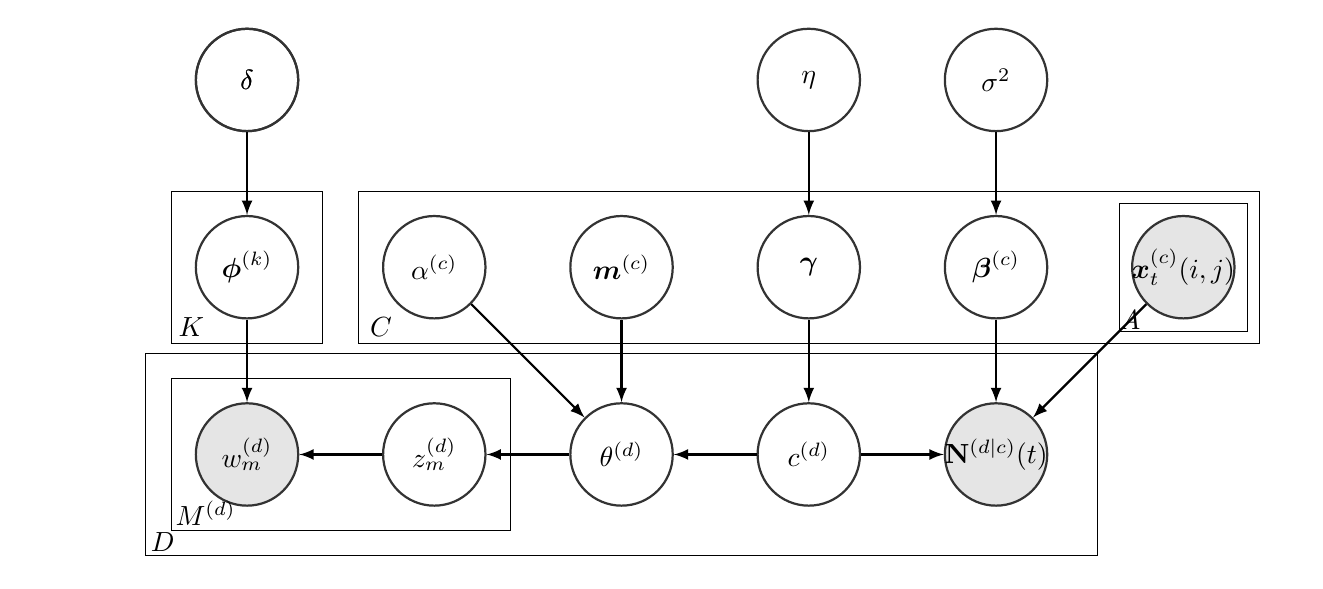
\begin{tikzpicture}
 	\tikzstyle{main}=[circle, minimum size = 13mm, thick, draw =black!80, node distance = 10.5mm]
 	\tikzstyle{connect}=[-latex, thick]
 	\tikzstyle{box}=[rectangle, draw=black!100]
 	\node[main, fill = white!100] (gamma) [label=center:$\boldsymbol{\gamma}$] { };
 	\node[main] (c) [below=of gamma,label=center:$c^{(d)}$] { };
 		\node[main, fill = black!10] (N) [right=of c ,label=center:$\mathbf{N}^{(d|c)}(t)$] { };	
 	 			\node[main] (eta) [above=of gamma,label=center:${\eta}$] { };
 	 	\node[main] (beta) [above=of N ,label=center:$\boldsymbol{\beta}^{(c)}$] { };
 	 	\node[main, fill = black!10] (x) [right=of beta ,label=center:$\boldsymbol{x}^{(c)}_t{(i,j)}$] { };
 	 		 	 								\node[main] (theta) [left=of c,label=center:${\theta}^{(d)}$] { };
 	 		 	 						 	 		\node[main] (sigma) [above=of beta,label=center:$\sigma^2$] { };
 	 		 	 						 	 		 		\node[main] (z) [left=of theta,label=center:$z_m^{(d)}$] {};
 	 		 	 						 	 		 		 	\node[main, fill = black!10] (w) [left=of z,label=center:$w_m^{(d)}$] { };
 	 		 	 						 	 		 		 	 	\node[main] (phi) [above=of w,label=center:$\boldsymbol{\phi}^{(k)}$] { };
 	 		 	 						 	 		 		 	 	 	\node[main] (delta) [above=of phi,label=center:$\delta$] { };
 	 		 	 						 	 		  	 		 	 							\node[main] (alpha) [above=of z,label=center:${\alpha}^{(c)}$] { };
 	 		 	 						 	 			 	 	 	\node[main] (delta) [above=of phi,label=center:$\delta$] { };
 	 		 	 						 	 			 	 	 	\node[main] (m) [above=of theta,label=center:$\boldsymbol{m}^{(c)}$] { };
 	\path (gamma) edge [connect] (c)
 	(z) edge [connect] (w)
 	(theta) edge [connect] (z)
 	(phi) edge [connect] (w)
 	(delta) edge [connect] (phi)
 	(sigma) edge [connect] (beta)
 	(x) edge [connect] (N)
 	(beta) edge [connect] (N)
 	(c) edge [connect] (N)
 	(c) edge [connect] (theta)
 	(alpha) edge [connect] (theta)
 	 	(m) edge [connect] (theta)
 		(eta) edge [connect] (gamma);
 			\node[rectangle, inner sep=2.5mm, fit=  (x),label=below left:$A$, xshift=5mm, yshift=5mm] {};
 			\node[rectangle, inner sep=3mm,draw=black!100, fit= (beta)(alpha) (m)(x)] {};
 				\node[rectangle, inner sep=4mm, fit= (beta)(alpha) (m)(x) ,label= below left:$C$, xshift=-41mm, yshift=5.5mm] {};
 	\node[rectangle, inner sep=3mm, draw=black!100, fit= (phi)] {};
 		\node[rectangle, inner sep=1.5mm, draw=black!100, fit= (x) ] {};
 		\node[rectangle, inner sep=0mm, fit= (phi),label=below left:$K$, xshift=2.5mm, yshift=1.5mm] {};
 	\node[rectangle, inner sep=0mm, fit= (w),label=below left:$M^{(d)}$, xshift=6.5mm, yshift=2mm] {};
 	\node[rectangle, inner sep=3mm,draw=black!100, fit= (w)(z)] {};
 	\node[rectangle, inner sep=3.5mm, fit= (c) (N) ,label=below left:$D$, xshift=-81mm, yshift=1.5mm] {};
 	\node[rectangle, inner sep=6.2mm, draw=black!100, fit =(c) (z) (w) (N) ] {};
 	\end{tikzpicture}}
 	\caption{Plate notation of IPTM}
 	\label{fig:plate}
 \end{figure}
 \begin{table}[ht]
 	 \centering
\scalebox{0.8}{ 	\begin{tabular}{ |c|c|c|} 
	\hline
 		\hline
 	Authors of the corpus &$\mathcal{A}$ & Set\\
 		\hline
 			Authors of the corpus given interaction pattern $c$ &$\mathcal{A}^{(c)}$ & Set\\
 			\hline
 	Number of authors &$A$ & Scalar \\
 		\hline
 		 	Number of documents &$D$ & Scalar \\
 		 	\hline
 		 	 	Number of words in the $d^{th}$ document &$M^{(d)}$ & Scalar \\
 		 	 	\hline
  	Number of topics & $K$ & Scalar \\
  	\hline
  	  Vocabulary size & $W$ & Scalar \\
  	  	\hline
  	 	Number of interaction patterns &$C$ & Scalar \\
  	 	\hline
  	 		Number of words assigned to interaction pattern and topic&$M^{CK}$ & Scalar \\
  	 		\hline
  	 			Number of words assigned to word and topic&$M^{WK}$ & Scalar \\
  	 			\hline
  	 	Interaction pattern of the $d^{th}$ document&$c^{(d)}$ & Scalar\\
  	 	\hline 
  	 	Time of the $d^{th}$ document&$t^{(d)}$ & Scalar\\
  	 		\hline 
  		Words in the $d^{th}$ document&$\boldsymbol{w}^{(d)}$ & $M^{(d)}$-dimensional vector\\
  		\hline 
  			$m^{th}$ word in the $d^{th}$ document&${w}_m^{(d)}$ & $m^{th}$  component of $\boldsymbol{w}^{(d)}$\\
  			\hline 	
  				Topic assignments in the $d^{th}$ document&$\boldsymbol{z}^{(d)}$ & $M^{(d)}$-dimensional vector\\
  				\hline 
  				Topic assignments for $m^{th}$ word in the $d^{th}$ document&${z}_m^{(d)}$ & $m^{th}$  component of $\boldsymbol{z}^{(d)}$\\
  				\hline 	
  				Dirichlet concentration prior given interaction pattern $c$&$\alpha^{(c)}$ & Scalar \\
  					\hline	
  				Dirichlet base prior given interaction pattern $c$&$\boldsymbol{m}^{(c)}$ & $K$-dimensional vector \\
  									\hline			
  							Dirichlet concentration prior&$\delta$ & Scalar \\
  							\hline			 
  								Dirichlet base prior&$\boldsymbol{n}$ & $W$-dimensional vector  \\
  								\hline				 	
  									Dirichlet concentration prior&$\eta$ & Scalar \\
  									\hline		
  										Dirichlet base prior&$\boldsymbol{l}$ & $C$-dimensional vector  \\
  										\hline			
  				Multinomial prior&$\gamma$ & $C$-dimensional vector \\
  				\hline
  				Variance of Normal prior&$\sigma^2$ & Scalar \\
  				\hline		
  					Probabilities of the words given topics &$\Phi$ & $W \times K$ matrix \\
  					\hline		
  						Probabilities of the words given topic $k$ &$\boldsymbol{\phi}^{(k)}$ & $W$-dimensional vector\\
  						\hline
  							Probabilities of the topics &$\Theta$ & $K \times D$ matrix \\
  							\hline		
  							Probabilities of the topics given the $d^{th}$ document &$\boldsymbol{\theta}^{(d)}$ & $K$-dimensional vector\\
  						\hline		
  						Coefficient of the intensity process given interaction pattern $c$ &$\boldsymbol{\beta}^{(c)}$ & $p$-dimensional vector\\
  							\hline		
  					Network statistics for directed edge $(i, j)$ given interaction pattern $c$ &$\boldsymbol{x}^{(c)}_t{(i,j)}$ & $p$-dimensional vector\\
  						\hline		
  				Counting process in the $d^{th}$ document given interaction pattern &	$\mathbf{N}^{(d|c)}(t)$ & $A\times A$ matrix\\
  						\hline
  						\hline
 	\end{tabular}}
 	\caption {Symbols associated with IPTM, as used in this paper}
 	\label{table:SymbolsIPTM}
 \end{table}
\normalsize
\clearpage
\subsection{Dynamic covariates to measure network effects}
The network statistics $\boldsymbol{x}^{(c)}_t(i, j)$ of Equation (2), corresponding to the ordered pair $(i, j)$, can be time-invariant (such as gender) or time-dependent (such as the number of two-paths from $i$ to $j$ just before time $t$). Since time-invariant covariates can be easily specified in various manners (e.g. homophily or group-level effects), here we only consider specification of dynamic covariates.
\begin{figure}[ht]
	\centering
	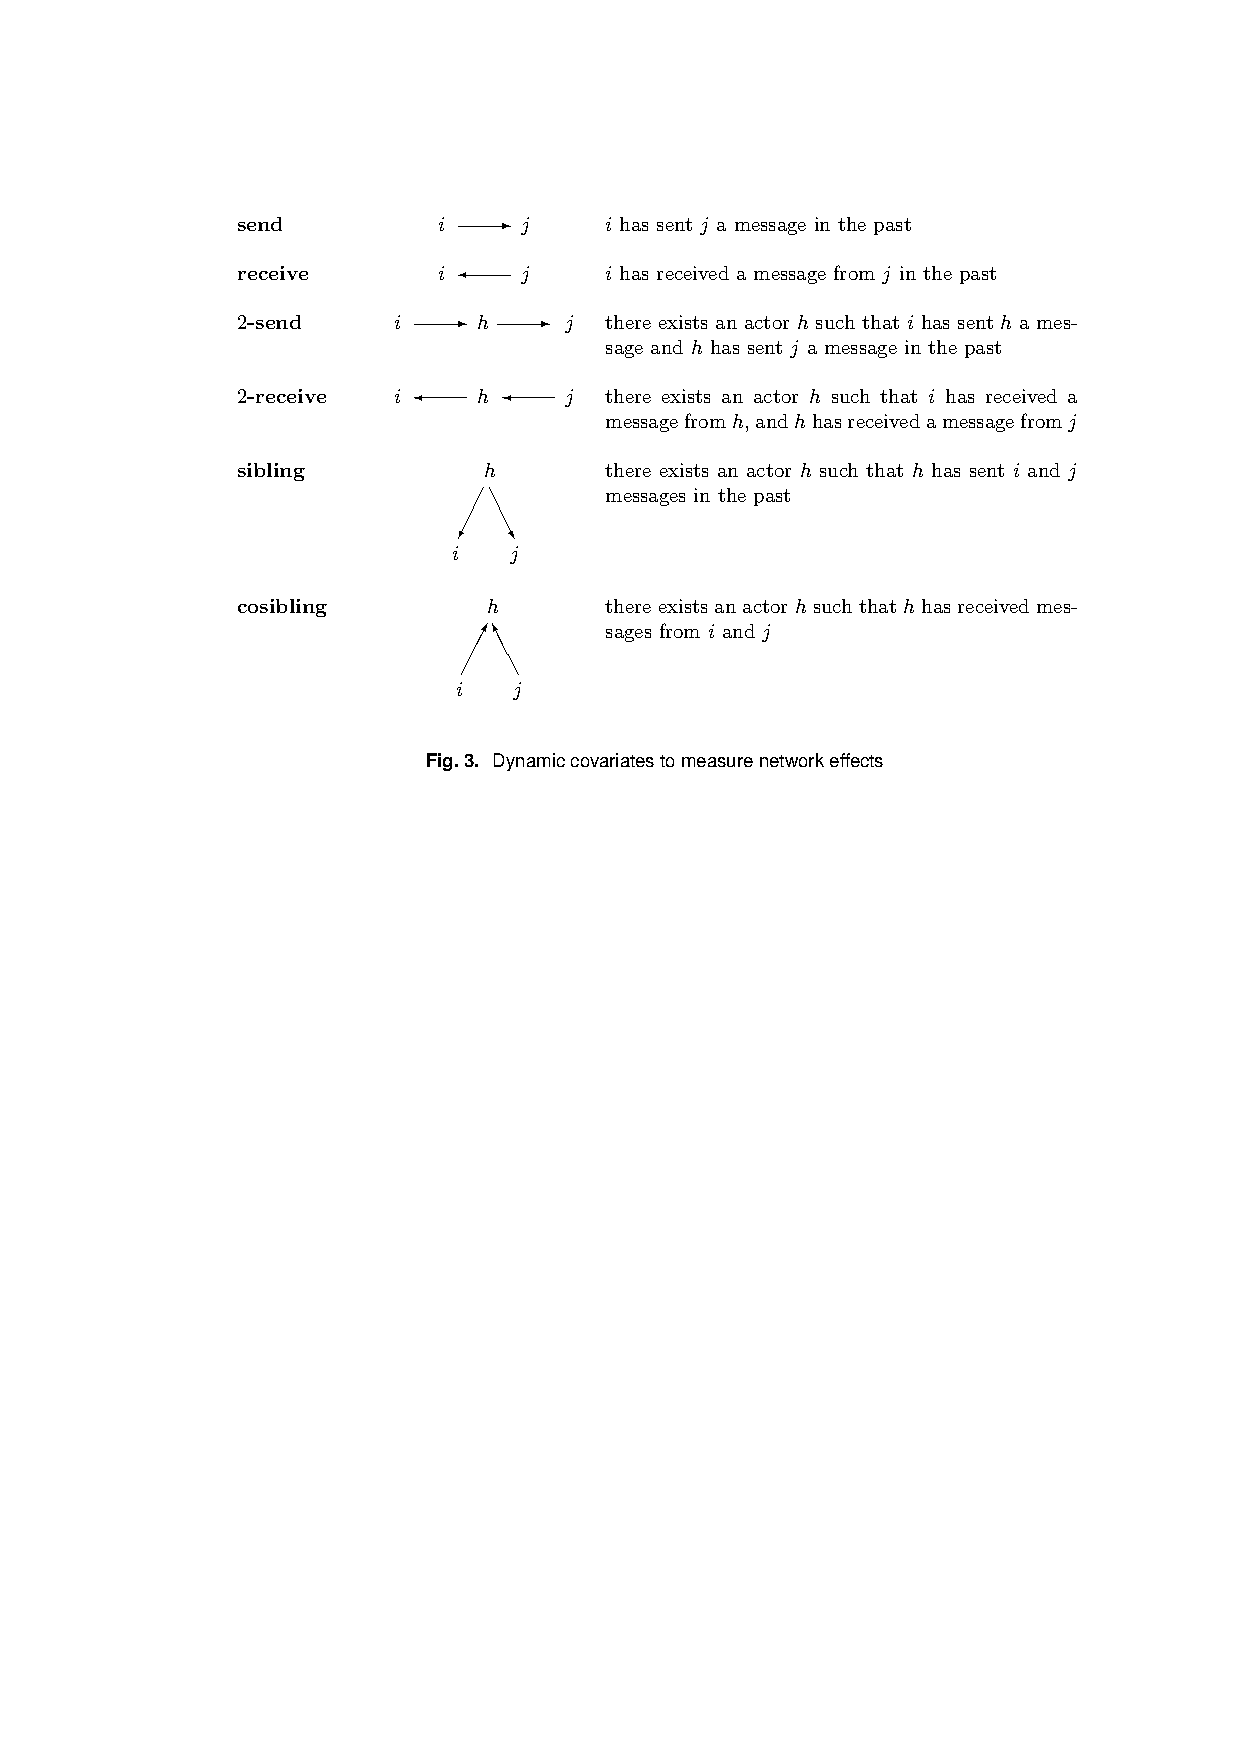
\includegraphics[width=0.56\textwidth]{PerryWolfe.pdf} 
	\label{fig:PerryWolfeplot}
\end{figure}
\newline Following \cite{PerryWolfe2012} (refer to Fig.3 of \cite{PerryWolfe2012} attached above), we use 4 effects as components of $\boldsymbol{x}^{(c)}_t(i, j)$, including the intercept to estimate the baseline intensities. The two behaviors (send and receive) are dyadic, involving exactly two actors,
while the one is triadic (sum of 2-send, 2-receive, sibling, and cosibling), involving exactly three actors. In addition to the ones from \cite{PerryWolfe2012}, we also include the indegree for receiver and outdegree for sender effects to measure the popularity and centrality. However, one different point from the existing specification is that we define the effects not to be based on finite sub-interval, which require large number of dimension. Instead, we create a single statistic for each effect by incorporating the recency of event into the statistic itself. As a result, all of the statistics can be seen as time-weighted dynamic network statistics.
\begin{itemize}[leftmargin=*,rightmargin=-1cm]
\item [1.] $\mbox{intercept}_t(i, j) = 1$
\item [2.]  $\mbox{send}_t(i, j)=\sum\limits_{d: t^{(d)}<t} I\{i\rightarrow j\}\cdot g(t-t^{(d)})$
\item [3.] $\mbox{receive}_t(i, j)=\sum\limits_{d: t^{(d)}<t} I\{j\rightarrow i\}\cdot g(t-t^{(d)})$
\item [4.] $\mbox{triangle}_t(i, j)=\sum\limits_{h \neq i, j}\Big(\sum\limits_{d: t^{(d)}<t}  I\{i\rightarrow h \mbox{ or } h\rightarrow j \}\cdot g(t-t^{(d)})\Big)\Big(\sum\limits_{d: t^{(d)}<t} I\{j\rightarrow h \mbox{ or } h\rightarrow j\}\cdot g(t-t^{(d)})\Big)$
\item [5.]  $\mbox{outdegree}_t(i)=\sum\limits_{j\neq i}\sum\limits_{d: t^{(d)}<t} I\{i\rightarrow j\}\cdot g(t-t^{(d)})$
\item [6.] $\mbox{indegree}_t(j)=\sum\limits_{i \neq j}\sum\limits_{d: t^{(d)}<t} I\{j\rightarrow i\}\cdot g(t-t^{(d)})$
\end{itemize}
Here, $g(t-t^{(d)})$ reflects the difference between current time $t$ and the timestamp of previous email $t^{(d)}$, thus measuring the recency. Inspired by the self-exciting Hawkes process, which is often used to model the temporal effect of email data, we can take the exponential kernel $g(t-t^{(d)})=e^{-\lambda(t-t^{(d)})}$ where $\lambda$ is the parameter of speed at
which sender replies to emails, with larger values indicating faster response times. Indeed, $\lambda^{-1}$ is the expected number of hours it takes to reply to a typical email. For simplicity, in our simulation we fixed $\lambda=0.05$ (i.e. $g(t-t^{(d)})=e^{-0.05(t-t^{(d)})}$), but this setup may vary based on the nature of document.
\section{Inference}
The inference for IPTM is similar to that of CPME. In this case, what we actually observe are the tokens $\mathcal{W}=\{\boldsymbol{w}^{(d)} \}_{d=1}^{D}$ and the sender, recipient, and timestamps of the email in the form of the counting process $\mathcal{N}=\{\boldsymbol{N}^{(d)}(t^{(d)}) \}_{d=1}^{D}.$ Next,  $\mathcal{X}=\{\boldsymbol{x}^{(c)}_{t^{(d)}}(i, j)\}_{d=1}^{D}$ is the metadata, and the latent variables are $\Phi=\{\boldsymbol{\phi}^{(k)}\}_{k=1}^{K}, \Theta=\{\boldsymbol{\theta}^{(d)} \}_{d=1}^{D}, \mathcal{Z}=\{\boldsymbol{z}^{(d)} \}_{d=1}^{D}, \mathcal{C}=\{{c}^{(d)} \}_{d=1}^{D},$ and $\mathcal{B}=\{\boldsymbol{\beta}^{(c)} \}_{c=1}^{C}$.\\
\newline 
Below is the the big joint distribution
\begin{equation}
\begin{aligned}
& P(\Phi, \Theta, \mathcal{W}, \mathcal{Z}, \mathcal{C}, \mathcal{B}, \mathcal{N}| \mathcal{X}, \delta, \boldsymbol{n}, \alpha, \boldsymbol{m}, \boldsymbol{\gamma}, \boldsymbol{\eta}, \sigma^2) \\& 
=  P(\mathcal{W}, \mathcal{Z}, \mathcal{C}, \mathcal{B}, \mathcal{N}| \Phi, \Theta, \mathcal{X}, \boldsymbol{\gamma}, \boldsymbol{\eta}, \sigma^2) P(\Phi, \Theta |\delta, \boldsymbol{n}, \alpha, \boldsymbol{m})
\\&= P( \mathcal{W}| \mathcal{Z}, \Phi)P(\mathcal{Z}|\Theta)P(\mathcal{N}|\mathcal{C}, \mathcal{X}, \mathcal{B})P(\mathcal{B}|\mathcal{C}, \sigma^2)P(\Phi|\delta, \boldsymbol{n})P(\Theta|\mathcal{C}, \alpha, \boldsymbol{m})P(\mathcal{C}|\boldsymbol{\gamma})P(\boldsymbol{\gamma}|\boldsymbol{\eta})
\end{aligned}
\end{equation}
Now we can integrate out $\Phi$ and $\Theta$ in latent Dirichlet allocation by applying Dirichlet-multinomial conjugacy as we did in CPME. See APPENDIX A for the detailed steps. After integration, we obtain below:
\begin{equation}
\propto P(\mathcal{W}|\mathcal{Z})P( \mathcal{Z}|\mathcal{C}, \delta, \boldsymbol{n}, \alpha, \boldsymbol{m})P(\mathcal{N}|\mathcal{C}, \mathcal{B}, \mathcal{X})P(\mathcal{B}|\mathcal{C}, \sigma^2)P(\mathcal{C}|\boldsymbol{\gamma})
\end{equation}
Then, we only have to perform inference over the remaining unobserved latent variables $\mathcal{Z}, \mathcal{C},$ and $\mathcal{B}$, using the equation below:
\begin{equation}
P( \mathcal{Z}, \mathcal{C}, \mathcal{B}|\mathcal{W}, \mathcal{N}, \mathcal{X}, \delta, \boldsymbol{n}, \alpha, \boldsymbol{m}, \boldsymbol{\gamma}, \boldsymbol{\eta}, \sigma^2) \propto P(\mathcal{W},  \mathcal{Z}, \mathcal{C}, \mathcal{B}, \mathcal{N} | \mathcal{X}, \delta, \boldsymbol{n}, \alpha, \boldsymbol{m}, \boldsymbol{\gamma}, \boldsymbol{\eta}, \sigma^2)
\end{equation}
 Either Gibbs sampling or Metropolis-Hastings algorithm is applied by sequentially resampling each latent variables from their respective conditional posterior.
  \subsection{Resampling $\mathcal{C}$}
   The first variable we are going to resample is the document-interaction pattern assignments, one document at a time. To obtain the Gibbs sampling equation, which is the posterior conditional probability for the interaction pattern $\mathcal{C}$ for $d^{th}$ document, i.e. $P(c^{(d)}=c|\mathcal{W}, \mathcal{Z},  \mathcal{C}_{\backslash d}, \mathcal{B}, \mathcal{N}, \mathcal{X}, \delta, \boldsymbol{n}, \alpha, \boldsymbol{m}, \boldsymbol{\gamma}, \boldsymbol{\eta}, \sigma^2)$. We can derive the equation as below:
  \begin{equation}
  \begin{aligned} & P(c^{(d)}=c|\mathcal{W}, \mathcal{Z}, \mathcal{C}_{\backslash d}, \mathcal{B}, \mathcal{N}, \mathcal{X}, \delta, \boldsymbol{n}, \alpha, \boldsymbol{m}, \boldsymbol{\gamma}, \boldsymbol{\eta}, \sigma^2)\\
  &\propto P(c^{(d)}=c, \boldsymbol{w}^{(d)}, \boldsymbol{z}^{(d)},  \mathbf{N}^{(d)}{(t^{(d)})}|\mathcal{W}_{\backslash d}, \mathcal{Z}_{\backslash d},\mathcal{C}_{\backslash d}, \mathcal{B}, \mathcal{N}_{\backslash d}, \mathcal{X}, \delta, \boldsymbol{n}, \alpha, \boldsymbol{m}, \boldsymbol{\gamma}, \boldsymbol{\eta}, \sigma^2)\\& \propto P(c^{(d)}=c|\mathcal{C}_{\backslash d}, \boldsymbol{\gamma}) P( \mathbf{N}^{(d)}{(t^{(d)})}| c^{(d)}=c, \mathcal{C}_{\backslash d}, \mathcal{B}, \mathcal{N}_{\backslash d}, \mathcal{X})P(\boldsymbol{w}^{(d)}, \boldsymbol{z}^{(d)}|c^{(d)}=c, \mathcal{W}_{\backslash d}, \mathcal{Z}_{\backslash d}, \mathcal{C}_{\backslash d}, \delta, \boldsymbol{n}, \alpha, \boldsymbol{m}), 
 \end{aligned}
  \end{equation}
 where $P(c^{(d)}=c|\mathcal{C}_{\backslash d}, \boldsymbol{\gamma})$ comes from the multinomial prior $\gamma$ and $P( \mathbf{N}^{(d)}{(t^{(d)})}| c^{(d)}=c, \mathcal{C}_{\backslash d}, \mathcal{B}, \mathcal{N}_{\backslash d}, \mathcal{X})$ is the probability of observing a document with the sender, receiver, and time equal to $(i=i^{(d)}, j=j^{(d)}, t=t^{(d)})$, respectively, given a set of parameter values. We will replace this by the partial likelihood in Equation (4) (without the product term since resampling of $c$ is document-specific). For the last term $P(\boldsymbol{w}^{(d)}, \boldsymbol{z}^{(d)}|c^{(d)}=c, \mathcal{W}_{\backslash d}, \mathcal{Z}_{\backslash d}, \mathcal{C}_{\backslash d}, \delta, \boldsymbol{n}, \alpha, \boldsymbol{m})$, we will follow typical LDA approach. \\ \newline Using Bayes' theorem (See APPENDIX B for conditional probabilty of the last term), we have
   \begin{equation}
   \begin{aligned} &=\Big[ \gamma_{c}\Big]\times\Big[ \frac{\mbox{exp}\{\boldsymbol{\beta}^{(c)T}x^{(c)}_{t^{(d)}}(i^{(d)}, j^{(d)})\}}{\sum_{j\in \mathcal{A}^{(c)}} \mbox{exp}\{\boldsymbol{\beta}^{(c)T}x^{(c)}_{t^{(d)}}(i^{(d)}, j)\}}\Big]\times\Big[\prod_{m=1}^{M^{(d)}}
    \frac{M_{z_m^{(d)}|d, \backslash d, m}+\alpha^{(c)} \boldsymbol{m}^{(c)}_{z_m^{(d)}}}{M_{\cdot|d}-1+\alpha^{(c)}}\Big],
   \end{aligned}
   \end{equation}
where $M_{k|d}$ is the number of times topic $k$ shows up in the document $d$. Furthermore, we can take the log of Equation (10) to avoid numerical issue from exponentiation and increase the speed of computation, which becomes:
  	 \begin{equation}
\mbox{log}(\gamma_{c})+\Big(\boldsymbol{\beta}^{(c)T}x^{(c)}_{t^{(d)}}(i^{(d)}, j^{(d)})-\mbox{log}\big[\sum_{j\in \mathcal{A}^{(c)}}\mbox{exp}\{\boldsymbol{\beta}^{(c)T}x^{(c)}_{t^{(d)}}(i^{(d)}, j)\}\big]\Big)+\sum_{m=1}^{M^{(d)}}\mbox{log}\Big(\frac{M_{z_m^{(d)}|d, \backslash d, m}+\alpha^{(c)} \boldsymbol{m}^{(c)}_{z_m^{(d)}}}{M_{\cdot|d}-1+\alpha^{(c)}}\Big).
  	 \end{equation}
  \subsection{Resampling $\mathcal{Z}$}
Next, the new values of $z^{(d)}_m$ are sampled for all of the token topic assignments (one token at a time), using the conditional posterior probability of being topic $k$ as we derived in APPENDIX B:
\begin{equation}
\begin{aligned} & 
 P(z^{(d)}_m=k|\mathcal{W}, \mathcal{Z}_{\backslash d, m},  \mathcal{C}, \mathcal{B}, \mathcal{N}, \mathcal{X}, \delta, \boldsymbol{n}, \alpha, \boldsymbol{m}, \boldsymbol{\gamma}, \boldsymbol{\eta}, \sigma^2)\\
& \propto P(z^{(d)}_m=k, w^{(d)}_m|\mathcal{W}_{\backslash d, m}, \mathcal{Z}_{\backslash d,m}, C, \delta, \boldsymbol{n}, \alpha, \boldsymbol{m})
\end{aligned}
\end{equation}
where the subscript $``{\backslash d, m}"$ denotes the exclsuion of position $m$ in email $d$. In the last line of equation (10), it is the contribution of LDA, so similar to CPME we can write the conditional probability:
	\begin{equation}
	\begin{aligned} 
	& \propto(M_{k|d, \backslash d, m}+\alpha^{(c^{(d)})} \boldsymbol{m}^{(c^{(d)})}_k)\times\frac{M_{w_m^{(d)}k, \backslash d, m}^{WK}+\delta n_w}{\sum_{w=1}^WM_{wk,  \backslash d, m}^{WK}+\delta}
	\end{aligned}
	\end{equation}
	which is the well-known form of collapsed Gibbs sampling equation for LDA.
\subsection{Resampling $\mathcal{B}$}
Finally, we wan to update the interaction pattern parameter $\boldsymbol{\beta}^{(c)}$, one interaction pattern at a time. For this, we will use the Metropolis-Hastings algorithm with a proposal density $Q$ being the multivariate Gaussian distribution, with variance $\delta^2_B$ (proposal distirbution variance parameters set by the
user), centered on the current values of $\boldsymbol{\beta}^{(c)}$. Then we draw a proposal $\boldsymbol{\beta}'^{(c)}$ at each iteration. Under symmetric proposal distribution (such as multivariate Gaussian), we cancel out Q-ratio and obtain the acceptance probability equal to:
\begin{equation}
\begin{split}
& \mbox{Acceptance Probability}=
\begin{cases}  \frac{P(\mathcal{B'}|\mathcal{W}, \mathcal{Z}, \mathcal{C}, \mathcal{N}, \mathcal{X})}{P(\mathcal{B}|\mathcal{W}, \mathcal{Z}, \mathcal{C}, \mathcal{N}, \mathcal{X})}\quad\text{if}  <1\\
1 \quad \text{else}
\end{cases}
\end{split}
\end{equation}
After factorization, we get
\begin{equation}
\begin{aligned}
\frac{P(\mathcal{B'}|\mathcal{W},\mathcal{Z}, \mathcal{C}, \mathcal{N}, \mathcal{X})}{P(\mathcal{B}|\mathcal{W}, \mathcal{Z}, \mathcal{C}, \mathcal{N}, \mathcal{X})} &=\frac{P(\mathcal{N}|\mathcal{B'}, \mathcal{W}, \mathcal{Z}, \mathcal{C}, \mathcal{X})P(\mathcal{B'})}{P(\mathcal{N}|\mathcal{B}, \mathcal{W}, \mathcal{Z},  \mathcal{C}, \mathcal{X})P(\mathcal{B})}\\&=\frac{P(\mathcal{N}|\mathcal{C}, \mathcal{X}, \mathcal{B'})P(\mathcal{B'})}{P(\mathcal{N}|\mathcal{C}, \mathcal{X}, \mathcal{B})P(\mathcal{B})},
\end{aligned}
\end{equation}
where $P(\mathcal{N}|\mathcal{C}, \mathcal{X}, \mathcal{B})$ is the partial likelihood in Equation (4).\\ \newline For $P(\mathcal{B})$, we select a multivarate Gaussian priors as mentioned earlier. Similar to what we did in Section 3.1, we can take the log and obtain the log of acceptance ratio as following:
\begin{equation}
\begin{aligned} 
&\mbox{log}\Big(\phi_d(\boldsymbol{\beta}^{\prime(c)};\mathbf{0}, \sigma^2I_P)\Big)-\mbox{log}\Big(\phi_d(\boldsymbol{\beta}^{\prime(c)};\mathbf{0}, \sigma^2I_P)\Big)\\&+\sum_{d:c^{(d)}=c}\Big\{\boldsymbol{\beta}^{\prime(c)T}x^{(c)}_{t^{(d)}}(i^{(d)}, j^{(d)})-\mbox{log}\big[\sum_{j\in \mathcal{A}^{(c)}}\mbox{exp}\{\boldsymbol{\beta}^{\prime(c)T}x^{(c)}_{t^{(d)}}(i^{(d)}, j)\}\big]\Big\}\\&-\sum_{d:c^{(d)}=c} \Big\{\boldsymbol{\beta}^{(c)T}x^{(c)}_{t^{(d)}}(i^{(d)}, j^{(d)})-\mbox{log}\big[\sum_{j\in \mathcal{A}^{(c)}}\mbox{exp}\{\boldsymbol{\beta}^{(c)T}x^{(c)}_{t^{(d)}}(i^{(d)}, j)\}\big]\Big\},
\end{aligned}
\end{equation}
where $\phi_d(\cdot;\mu, \Sigma)$ is the $d$-dimensional multivariate normal density.
Then the log of acceptance ratio we have is:
\begin{equation}
\mbox{log(Acceptance Probability) = min((16), 0) }
\end{equation}
To determine whether we accept the proposed update or not, we take the usual approach, by comparing the log of acceptance ratio we have to the log of a sample from uniform(0,1).\\
\subsection{Pseudocode}
To implement the inference procedure outlined above, we provide a pseudocode for Markov Chain Monte Carlo (MCMC) sampling. Note that we use two loops, outer iteration and inner iteration, in order to avoid the label switching problem \citep{jasra2005markov}, which is an issue caused by the nonidentifiability of the components under symmetric priors in Bayesian mixture modeling. When summarizing model results, we will only use the values from the last $I^{th}$ outer loop because there is no label switching problem within the inner iteration.
 \begin{algorithm}[H]
 	\SetAlgoLined
 	\caption{MCMC($I, n_1, n_2, n_3, \delta_B$ )}
    set initial values $\mathcal{C}^{(0)}, \mathcal{Z}^{(0)},$ and $\mathcal{B}^{(0)}$\\
 	\For{i=1 to I}{
 		\For{n=1 to $n_1$}{
 			fix $\mathcal{Z}=\mathcal{Z}^{(i-1)}$ and $\mathcal{B}=\mathcal{B}^{(i-1)}$ \\
 		  \For{d=1 to D}{
 		  	calculate $\boldsymbol{x}^{*(c)}_{t^{(d)}}(i^{(d)}, j)$ according to Section 2.3, for every $c=1,...,C$\\
	 		 calculate $p^\mathcal{C}|\boldsymbol{z}^{(d)}, \boldsymbol{\beta}^{(c^{(d)})}=(p_1,...,p_C),$ where $p_c=$ exp(Eq. (11) corresponding to $c$)\\
 		  	draw $c^{(d)}\sim \mbox{multinomial}(p^\mathcal{C})$}}
 		\For{n=1 to $n_2$}{
 			fix $\mathcal{C}=\mathcal{C}^{(i)}$ and $\mathcal{B}=\mathcal{B}^{(i-1)}$ \\
 			\For{d=1 to D}{
 		 \For{m=1 to $M^{(d)}$}{
 		 	calculate $p^\mathcal{Z}|\boldsymbol{c}^{(d)}, \alpha^{(c^{(d)})}, \boldsymbol{m}^{(c^{(d)})},  \boldsymbol{\beta}^{(c^{(d)})}=(p_1,...,p_K),$ where $p_k=$ exp(Eq. (13) corresponding to $k$)\\
 		 	 draw of $z_m^{(d)}\sim\mbox{multinomial}(p^\mathcal{Z})$}}
 		}
 			\For{n=1 to $n_3$}{
 				fix $\mathcal{C}=\mathcal{C}^{(i)}$, $\mathcal{Z}=\mathcal{Z}^{(i)}$, and $\mathcal{B}^{(0)}=$ last value ($n_3^{th}$) of $\mathcal{B}^{(i-1)}$\\
 				calculate $\mathcal{X}=\{\boldsymbol{x}^{*(c)}_{t^{(d)}}(i, j)\}_{d=1}^{D}$ according to Section 2.3, given fixed $\mathcal{C}$\\
 				 \For{c=1 to C}{draw $\boldsymbol{\beta}^{(c)}| \mathcal{C}, \mathcal{Z}, \mathcal{B}^{(n-1)}$ using M-H algorithm in Section 3.3}
 		 }
}	summarize the results using:\\ the last value of $\mathcal{C}$, the last value of $\mathcal{Z}$, and the last $n_3$ length chain of $\mathcal{B}$
 	\end{algorithm}
\subsection{Asymmetric Dirichlet prior over $\Theta$ (topic distribution)}
\cite{wallach2009rethinking} demonstrated that the typical implementations of topic models using symmetric Dirichlet priors with fixed concentration parameters often result in less practical results, and the model fitting can be improved by applying an asymmetric Dirichlet prior over the document–topic distributions (i.e. $\Theta$). Therefore, we assign an asymmetric Dirichlet prior over the interaction pattern-topic distributions, $\Theta=\{\boldsymbol{\theta}^{(d)} \}_{d=1}^{D}$, where $\boldsymbol{\theta}^{(d)}$ is drawn from Dir($\alpha^{(c^{(d)})}, \boldsymbol{m}^{(c^{(d)})}$). While \cite{wallach2009rethinking} illustrates two different methods, adding a hierarchy to $\Theta$ and optimizing the hyperparameters ($\alpha$ and $\boldsymbol{m}$), we choose to use hyperparameter
optimization steps since it is computationally efficient and also sufficient to achieve the desired performance gains. Now, we assume $\boldsymbol{m}^{(c)}$ to be non-uniform base measures (while $\alpha^{(c)}$ is still a fixed concentration parameter), and implement the hyperparameter optimization technique called ``new fixed-point iterations using the Digamma recurrence relation'' in \cite{wallach2008structured} based on Minka’s fixed-point iteration \citep{minka2000estimating}.\\ \newline
Here we summarize Chapter 2 of \cite{wallach2008structured} and its extension to our IPTM, to illustrate the basic steps and equations used for our optimization. Basically, we want to find the optimal hyperparameter $[\alpha\boldsymbol{m}]^*$ given the data $\mathcal{D}$ such that the probability of the
data given the hyperparameters $P(\mathcal{D}|\alpha\boldsymbol{m})$ is maximized at $[\alpha\boldsymbol{m}]^*$. After incorporating the interaction pattern component, the evidence is now given by 
\begin{equation}
P(\mathcal{D}^{(c)}|\alpha^{(c)}\boldsymbol{m}^{(c)})=\prod_{d:c^{(d)}=c} \frac{\Gamma(\alpha^{(c)})}{\Gamma(M_{\cdot|d}+\alpha^{(c)})}\prod_{k=1}^{K}\frac{\Gamma(M_{k|d}+\alpha^{(c)} m^{(c)}_k)}{\Gamma(\alpha^{(c)} m^{(c)}_k)}
\end{equation} and is concave in $\alpha^{(c)} \boldsymbol{m}^{(c)}$, thus we will estimate $[\alpha^{(c)}\boldsymbol{m}^{(c)}]^*$ within each outer runs of MCMC.\\
\newline First, the starting point is derived by Minka’s fixed-point iteration which takes the derivative of the lower bound $B([\alpha^{(c)}\boldsymbol{m}^{(c)}]^*)$ of $\mbox{log}P(\mathcal{D}^{(c)}|[\alpha^{(c)}\boldsymbol{m}^{(c)}]^*)$ with respect to $[\alpha^{(c)} {m^{(c)}_k}]^*$:
\begin{equation}
[\alpha^{(c)} m^{(c)}_k]^*=\alpha^{(c)} m^{(c)}_k\frac{\sum_{d:c^{(d)}=c}\Psi(M_{k|d}+\alpha^{(c)} m^{(c)}_k)-\Psi(\alpha^{(c)} m^{(c)}_k)}{\sum_{d:c^{(d)}=c}\Psi(M_{\cdot|d}+\alpha^{(c)})-\Psi(\alpha^{(c)})},
\end{equation}
where $\Psi(\cdot)$ is the first derivative of the log gamma function, known as the digamma function, and the quantity $M_{k|d}$ is the number of times that outcome $k$ was observed in the document $d$. Moreover, the quantity $M_{\cdot|d}=\sum_{k=1}^K M_{k|d}$ is the total number of words in the document $d$. The
value $\alpha^{(c)} m^{(c)}_k$ acts as an initial “pseudocount” for outcome $k$ across the documents of interaction pattern $c$.\\ \newline
Next, Wallach's new method rewrites the equation above using the notation $C_k(n)=\sum\limits_{d:c^{(d)}=c}\delta(M_{k|d}-n)$ and $C_\cdot(n)=\sum\limits_{d:c^{(d)}=c}\delta(M_{\cdot|d}-n)$:
\begin{equation}
[\alpha^{(c)} m^{(c)}_k]^*=\alpha^{(c)} m^{(c)}_k\frac{\sum_{n=1}^{\mbox{max}_dM_{k|d}}C_k(n)[\Psi(n+\alpha^{(c)} m^{(c)}_k)-\Psi(\alpha^{(c)} m^{(c)}_k)]}{\sum_{n=1}^{\mbox{max}_dM_{\cdot|d}}C_\cdot(n)[\Psi(n+\alpha^{(c)})-\Psi(\alpha^{(c)})]}.
\end{equation}
Finally, applying the digamma recurrence relation (for any positive integer $n$) $$\Psi(n+z)-\Psi(z)=\sum_{f=1}^{n}\frac{1}{f-1+z},$$ we subtitute Equation (20) for below:
\begin{equation}
[\alpha^{(c)} m^{(c)}_k]^*=\alpha^{(c)} m^{(c)}_k\frac{\sum_{n=1}^{\mbox{max}_dM_{k|d}}C_k(n)\sum_{f=1}^n \frac{1}{f-1+\alpha^{(c)} m^{(c)}_k}}{\sum_{n=1}^{\mbox{max}_dM_{\cdot|d}}C_\cdot(n)\sum_{f=1}^n \frac{1}{f-1+\alpha^{(c)}}}.
\end{equation}
This method is as accurate as Mika's fixed-point iteration method, but it acheives computational efficiency since the digamma recurrence relation reduces the number of new calculations required for each successive $n$ to one. Pseudocode
for the complete fixed-point iteration is given in algorithm 2.2 of \cite{wallach2008structured}.
\section{Appliction to North Carolina email data}
To see the applicability of the model, we used the North Carolina email data using two counties, Vance county and Dare county, which are the two counties whose email corpus cover the date of Hurricane Sandy (October 22, 2012 – November 2, 2012). Exploratory analysis revealed that Dare county experienced significant change in the pattern of email exchanges; specifically, during the emergency period, email interactions significanty less rely on previous history of interactions, compared to the normal period. On the other hand, Vance county did not experience any distinctive change, and the possible reason for the difference is the locations of two counties. Here we apply IPTM to both data to see the differences in detail, in terms of the interaction patterns and topics of the corpus.
\subsection{Vance county email data}
After treating multicast emails (those involving a single sender but multiple receivers) as multiple distinct emails, Vance county data contains 269 emails (only count the email with the number of words greater than 0) between 18 actors, including 620 vocabulary in total. We used $K=10$ topics and $C=3$ interaction patterns, with the parameters fixed as $\alpha=50/K=50/10=5$ with $\boldsymbol{m}=(1,...,1)^T/K$ ($\alpha$ and $\boldsymbol{m}$ are fixed only at the initial step), $\delta=0.01$, and $\eta=50/C=50/3=16.67$, following the common practice. The asymmetric model uses same $\delta$ and $\eta$, but $\alpha^{(c)}$ and $\boldsymbol{m}^{(c)}$ are optimized for every outer iteration, for every interaction pattern. \\ \newline MCMC sampling was implemented based on the order and scheme illustrated in Section 3. We set the outer iteration number as $I=500$, the inner iteration numbers as $n_1=3, n_2=3,$ and $n_3=3300$. First 50 outer iterations and first 300 iterations of third inner iteration were used as a burn-in, and every $3^{rd}$ sample was taken as a thinning process of third inner iteration. In addition, after some experimentation, $\delta_B$ was set as 0.5, to ensure sufficient acceptance rate. As demonstrated in Algorithm 5, the last value of $\mathcal{C}$, the last value of $\mathcal{Z}$, and the last $n_3$ length chain of $\mathcal{B}$ were taken as the final posterior samples. After these post-processing, MCMC diagnostic plots are attached in APPENDIX C, as well as the geweke test statistics. \\\newline
Below are the summary of IP-topic-word assignments. Each interaction pattern is paired with (a) posterior estimates of dynamic network effects $\boldsymbol{\beta}^{(c)}$ corresponding to the interaction pattern, (b) the top 3 topics most likely to be generated conditioned on the interaction pattern, and (c) the top 10 most likely words to have generated conditioned on the topic and interaction pattern.
\begin{table}[ht]
	\centering
	\begin{tabular}{|c|c|c|c|} 
		\hline
		& \textbf{IP1} (54 emails) & \textbf{IP2} (107 emails) &\textbf{IP3} (108 emails) \\
		\hline
		\textbf{intercept} & 0.515 [-0.523, 1.546]& -0.364 [-2.108, 1.934]& -1.230 [-1.948, 0.194]\\
		\textbf{send}&  1.916* [1.130, 2.937]& 2.843* [1.969, 3.885]& 2.531* [1.595, 3.568]\\
		\textbf{receive}& 0.158 [-1.126, 1.098]& 3.068* [2.427, 4.509]& 1.067* [0.488, 1.781]\\
		\textbf{triangles} & 1.483 [-0.507, 2.558]& -1.478* [-2.038, -0.918]& -1.787* [-3.062, -0.958]\\
		\textbf{outdegree} & 0.514 [-0.570, 1.377]& 0.492 [-0.804, 1.665]& 0.771 [-1.152, 2.544]\\
		\textbf{indegree} & 2.166* [1.534, 2.895]& 1.397* [0.720, 2.187]& 2.464* [1.840, 3.327]\\
						\hline
	\end{tabular}
	\caption {Summary of posterior estimates of $\boldsymbol{\beta}^{(c)}$ for Vance county emails}
	\label{table:Vancebeta}
\end{table}
\begin{figure}[ht]
	\centering
	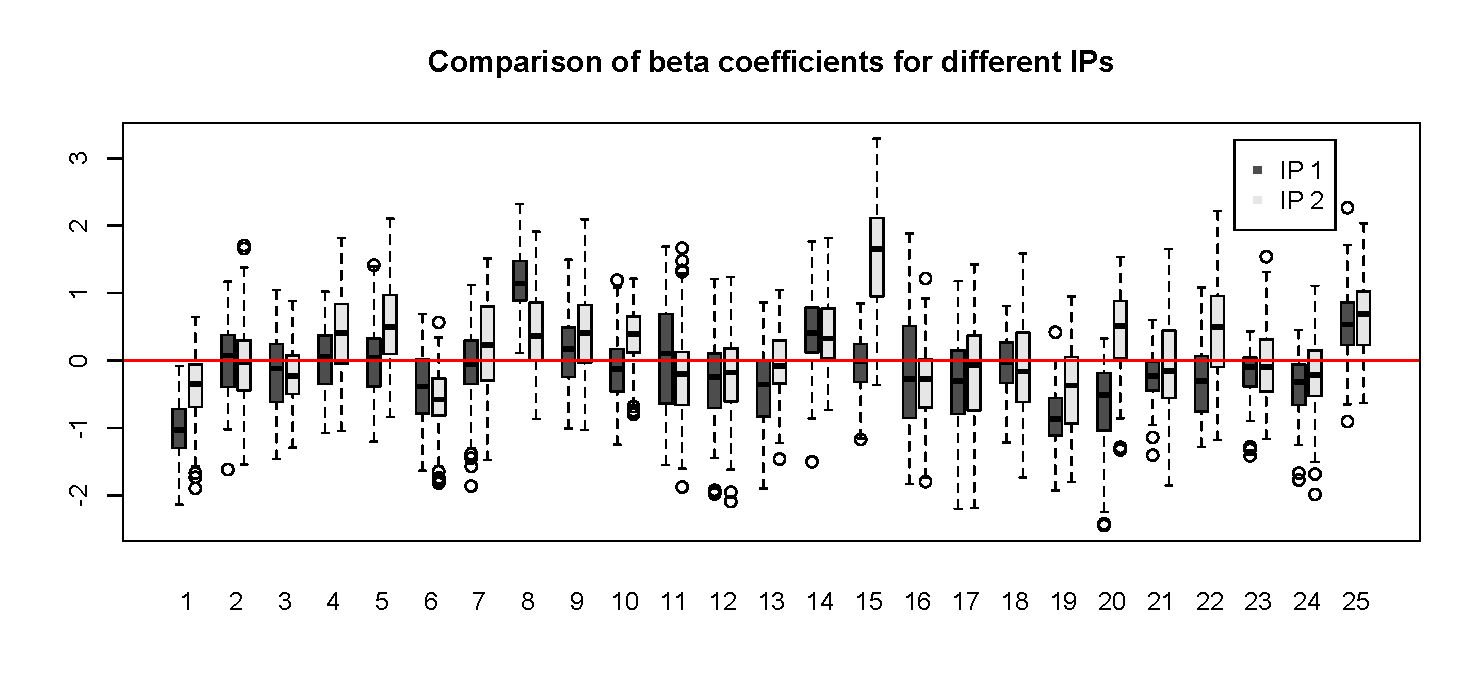
\includegraphics[width=1\textwidth]{betaplot.pdf} 
	\caption{Posterior distribution of  $\boldsymbol{\beta}^{(c)}$ for Vance county emails}
	\label{fig:Vanceboxplot}
\end{figure}
\begin{comment}
\newline First, Table 2 summarizes the posterior means and 95\% credible interval for $\boldsymbol{\beta}^{(c)}$ corresponding to each interaction patterns. Below are the several examples of the interpretation of estimates, in the context of point process framework in Section 2.1. The interpretation can be extended to any other interaction patterns and time intervals between the two emails.
\begin{itemize} 
	\item (\textbf{Intercept}) Assuming no history at all between the sender and receiver, the document is $\frac{e^{(0.014)}}{e^{(-0.110)}}\approx 1.132$ times more likely to be IP3 relative to IP1, $\frac{e^{(0.014)}}{e^{(-0.189)}}\approx 1.225$ times more likely to be IP3 relative to IP2, and $\frac{e^{(-0.110)}}{e^{(-0.189)}}\approx 1.082$ times more likely to be IP2 relative to IP1
	\item (\textbf{Send}) If $i$ sends an email to $j$ at time $t$, the likelihoods of $i$ sends email of IP1 to $j$ after 1 hour and 2 hours are multiplied by $e^{(2.345\times e^{(-0.05)})}\approx 9.306$ and $e^{(2.345\times e^{(-2\times 0.05)})}\approx 8.347$, respectively.
	\item (\textbf{Receive}) If $j$ sends an email to $i$ at time $t$, the likelihoods of $i$ sends email of IP1 to $j$ after 30 minutes and 30 hours are multiplied by $e^{(1.530\times e^{(-0.5\times 0.05)})}\approx 4.447$ and $e^{(1.530\times e^{(-30\times 0.05)})}\approx 1.407$, respectively.
	\item (\textbf{Triangles}) If $i$ sends/receives an email to/from $k$ at time $t$, and $k$ sends/receives an email to/from $j$ at time $t+1$ (i.e. after 1 hour from $t$), then $i$ sends/receives email to/from $j$ at time $t+2$ (i.e. after 2 hour from $t$) at a slightly higher rate if IP1 (likelihood multiplied by $e^{(0.589\times e^{(-1)}\times e^{(-1)})}\approx 1.083$).
\end{itemize}
\end{comment}
By examining the estimates in Table 2 and their corresponding interpretaiton, it seems that there exist strong effects of dynamic network covariates. That is, whether the sender and receiver previously had dyadic or triangle interaction strongly increase the rate of their interactions. Moreover, to see the differences across the interaction patterns more clearly, we compared the posterior distribution using the boxplots in Figure 2 and it seems that there exists notable differences in dynmic network covariates across the interaction patterns. For example, IP2 has the highest send and receive effect and IP3 has the highest outdegree and indegree effect, while its baseline intensity (i.e. intercept) or triangle effect are not as high as other interaction patterns. Later, multiple hypothesis testing could be applied in order to test the significance of the differences in  $\boldsymbol{\beta}^{(c)}$ across the $C$ number of interaction patterns.\\\newline
Next, we scrutinize the topic distributions corresponding to each interaction patterns in Figure 3. There is some distinctive differences in the topic distributions $\mathcal{Z}$, given the assignment of interaction patterns to the documents $\mathcal{C}$. Specifically, each interaction pattern has different topics as the topic with highest probability.
\begin{figure}[ht]
	\centering
	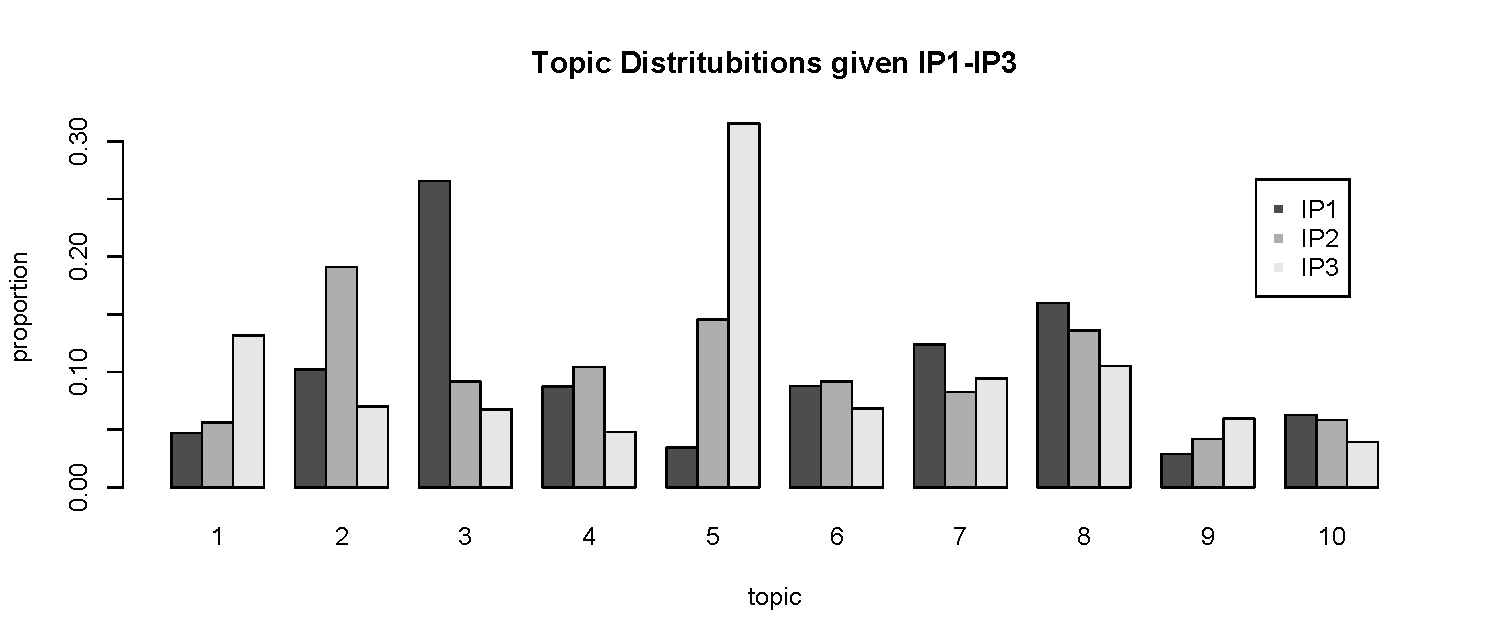
\includegraphics[width=1\textwidth]{topicplot.pdf} 
		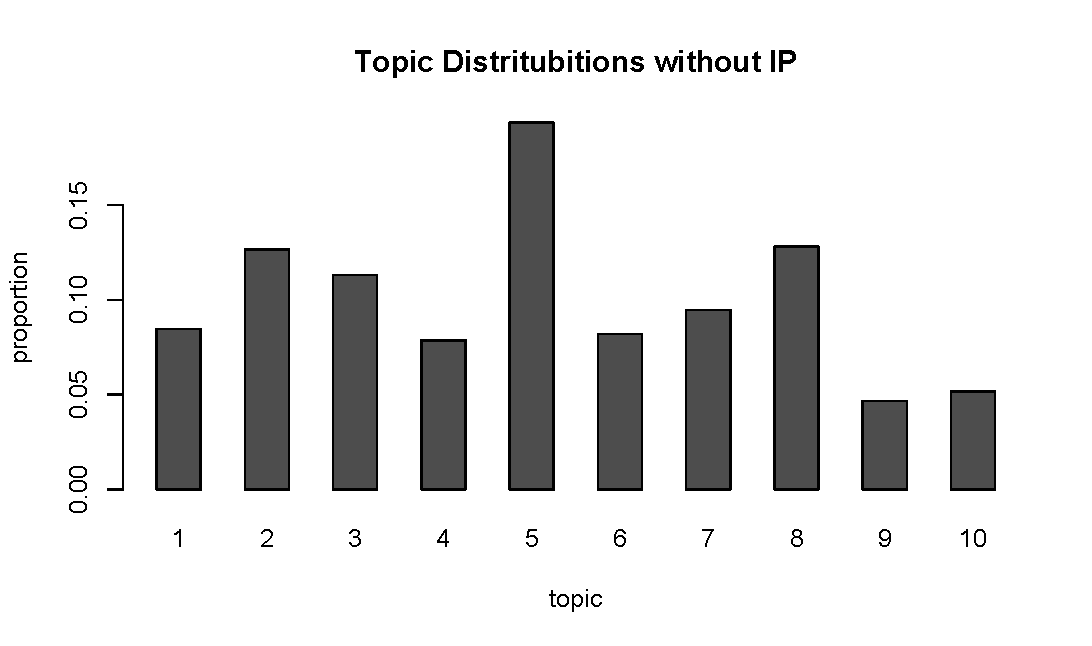
\includegraphics[width=1\textwidth]{topicplot2.pdf} 
	\caption{Posterior distribution of  $\mathcal{Z}$ for Vance county emails, with (upper) and without (lower) considering IP}
	\label{fig:Vancebarplot}
\end{figure}
\normalsize
\newline
Furthermore, we look at the distribution of words given the topics, which corresponds to Algorithm 4 in the generative process. Since the topic-word distribution $\phi$ does not depend on the interaction patterns as previous cases, Table 3 lists top 10 topics with top 10 words that have the highest probability conditioned on the topic. In addition, this time we try to check the interaction pattern-word distribution by listing top 10 words that have the highest probability conditioned on the interaction pattern. It seems that the words are not significantly different, having several words like `director', `phones', `department', `description', or `henderson' (county seat of Vance county) appeared repetitively across the most of the topics or interaction patterns. The word 'will' was ranked the top in most of the lists, probably because it was not deleted during the text mining process while other similar type of words like `am', `is', `are', or `can' are all removed. \\
		\begin{table}[ht]
			\centering
\begin{tabular}{|l||l||l|}
					\hline
					{\textbf{IP1} (54 emails)}&{\textbf{IP2} (107 emails)}&{\textbf{IP3} (108 emails)}\\
					\hline\hline
					K=2 (0.40), K=4 (0.17), K=9 (0.15) & K=8 (0.38), K=5 (0.24)& K=1 (0.31), K=3 (0.17), K=6 (0.15)\\
					\hline
					message, electronic, records&phones, phone& henderson, street, description\\
					time, response, ncgs & week, department& latest, fax, church\\
					department, hereto, attachments& system, rest& planning, suite, emergency\\
					heads, finance, director& october, advised& attached, director, center\\
					request, financial, operations& training, jail& extension, goldvancesealimprovedjordan, phone\\
					manager, system, work& cutting, send& development, phase, morning\\
					pursuant, additional, office & cutover, center& e-mail, board, email\\
					chapter, class, helped& folks, tuesday& good, rural, excel\\ 
					public, local, internal& instructions, monday& young, funds, lease\\
					subject, communications, reporting& dss, thursday& list, turn, form\\
					\hline
				\end{tabular}
				\caption {Summary of top 5 topics with top 10 words that have the highest probability conditioned on the topic (Symmetric)}
				\label{table:VancewordsMCMC}
			\end{table}
\begin{comment}
\begin{table}[ht]
	\centering
	\scalebox{0.9}{	\begin{tabular}{|l|l||l|l||l|l||l|l||l|l|}
			\hline
			\multicolumn{2}{|l||}{\textbf{Topic 9} (0.0946)}&\multicolumn{2}{l||}{\textbf{Topic 19} (0.0907)}&\multicolumn{2}{l||}{\textbf{Topic 2} (0.0869)}&\multicolumn{2}{l||}{\textbf{Topic 13} (0.0849)}&\multicolumn{2}{l|}{\textbf{Topic 8} (0.0671)}\\
			\hline\hline
			\scriptsize will&\scriptsize 0.0622&\scriptsize will&\scriptsize 0.0487&\scriptsize will&\scriptsize 0.709&\scriptsize will&\scriptsize 0.0237&\scriptsize will&\scriptsize 0.0419\\
			\scriptsize suite&\scriptsize 0.0184&\scriptsize director&\scriptsize  0.0428&\scriptsize director&\scriptsize 0.0370&\scriptsize street&\scriptsize 0.0221&\scriptsize system&\scriptsize 0.0279\\
			\scriptsize henderson&\scriptsize  0.0170&\scriptsize description&\scriptsize 0.0310&\scriptsize department&\scriptsize 0.0277&\scriptsize phones&\scriptsize 0.0189&\scriptsize phones&\scriptsize 0.0259\\
			\scriptsize october&\scriptsize 0.0170&\scriptsize message&\scriptsize 0.0206&\scriptsize henderson&\scriptsize 0.0200&\scriptsize  october&\scriptsize 0.0173&\scriptsize director&\scriptsize 0.0200\\
			\scriptsize system&\scriptsize 0.0170&\scriptsize phones&\scriptsize  0.0177&\scriptsize center&\scriptsize0.0154&\scriptsize fax&\scriptsize 0.0158&\scriptsize center&\scriptsize 0.0180\\
			\scriptsize extension&\scriptsize 0.0156&\scriptsize meeting&\scriptsize 0.0162&\scriptsize phone&\scriptsize 0.0154&\scriptsize suite&\scriptsize 0.0158&\scriptsize  emergency&\scriptsize 0.0160\\
			\scriptsize meeting&\scriptsize 0.0156&\scriptsize fax&\scriptsize  0.0147&\scriptsize october&\scriptsize 0.0139&\scriptsize church&\scriptsize 0.0142&\scriptsize october&\scriptsize 0.0160\\
			\scriptsize phone&\scriptsize 0.0156&\scriptsize latest&\scriptsize  0.0147&\scriptsize street&\scriptsize 0.0139&\scriptsize phone&\scriptsize 0.0142&\scriptsize  attached&\scriptsize 0.0140\\
			\scriptsize electronic&\scriptsize 0.0141&\scriptsize october&\scriptsize  0.0147&\scriptsize church&\scriptsize 0.0123&\scriptsize advised&\scriptsize 0.0139&\scriptsize  department&\scriptsize 0.0140\\
			\scriptsize heads&\scriptsize 0.0141&\scriptsize street&\scriptsize  0.0147&\scriptsize fax&\scriptsize 0.0123&\scriptsize heads&\scriptsize 0.0126&\scriptsize message&\scriptsize0.0140\\
			\hline\hline
			\multicolumn{2}{|l||}{\textbf{Topic 15} (0.0628)}&\multicolumn{2}{l||}{\textbf{Topic 7} ( 0.0566)}&\multicolumn{2}{l||}{\textbf{Topic 3} (0.0435)}&\multicolumn{2}{l||}{\textbf{Topic 6} (0.0427)}&\multicolumn{2}{l|}{\textbf{Topic 16} (0.0400)}\\
			\hline\hline
			\scriptsize will&\scriptsize 0.0554&\scriptsize henderson&\scriptsize 0.0378&\scriptsize heads&\scriptsize 0.0308&\scriptsize department&\scriptsize 0.0502&\scriptsize operations&\scriptsize 0.0268\\
			\scriptsize henderson&\scriptsize 0.0256&\scriptsize will&\scriptsize  0.0355&\scriptsize will&\scriptsize 0.0277&\scriptsize will&\scriptsize 0.0408&\scriptsize phone&\scriptsize 0.0268\\
			\scriptsize phones&\scriptsize 0.0256&\scriptsize phone&\scriptsize 0.0307&\scriptsize director&\scriptsize 0.0246&\scriptsize director&\scriptsize 0.0345&\scriptsize system&\scriptsize 0.0268\\
			\scriptsize phone&\scriptsize 0.0192&\scriptsize church&\scriptsize 0.0189&\scriptsize street&\scriptsize 0.0215&\scriptsize phone&\scriptsize 0.0251&\scriptsize department&\scriptsize 0.0234\\
			\scriptsize street&\scriptsize 0.0192&\scriptsize coming&\scriptsize 0.0189&\scriptsize directory&\scriptsize 0.0185&\scriptsize electronic&\scriptsize 0.0219&\scriptsize church&\scriptsize 0.0201\\
			\scriptsize suite&\scriptsize 0.0192&\scriptsize phones&\scriptsize 0.0189&\scriptsize phone&\scriptsize 0.0185&\scriptsize week&\scriptsize 0.0219&\scriptsize director&\scriptsize 0.0201\\
			\scriptsize cutting&\scriptsize 0.0171&\scriptsize suite&\scriptsize 0.0165&\scriptsize  attached&\scriptsize 0.0154&\scriptsize church&\scriptsize 0.0157&\scriptsize message&\scriptsize 0.0201\\
			\scriptsize department&\scriptsize 0.0171&\scriptsize training&\scriptsize 0.0165&\scriptsize days&\scriptsize 0.0154&\scriptsize description&\scriptsize 0.057&\scriptsize phones&\scriptsize 0.0201\\
			\scriptsize electronic&\scriptsize 0.0149&\scriptsize  attached&\scriptsize 0.0142&\scriptsize description&\scriptsize 0.0154&\scriptsize development&\scriptsize 0.0157&\scriptsize will&\scriptsize 0.0201\\
			\scriptsize rest&\scriptsize 0.0149&\scriptsize description&\scriptsize  0.0142&\scriptsize e-mail&\scriptsize 0.0154&\scriptsize emergency&\scriptsize 0.0157&\scriptsize directory&\scriptsize0.0167\\
			\hline
		\end{tabular}}
		\caption {Summary of top 10 topics with top 10 words that have the highest probability conditioned on the topic}
		\label{table:VancewordsMCMC}
	\end{table}
	\normalsize
	\begin{table}[ht]
		\centering
		\scalebox{0.9}{	\begin{tabular}{|l|l||l|l||l|l|}
				\hline
				\multicolumn{2}{|l||}{\textbf{IP1} (0.4721)}&\multicolumn{2}{l||}{\textbf{IP2} (0.2082)}&\multicolumn{2}{l||}{\textbf{IP3} (0.3197)}\\
				\hline\hline
				\scriptsize will&\scriptsize 0.0505&\scriptsize will&\scriptsize 0.0551&\scriptsize director&\scriptsize 0.257\\
				\scriptsize director&\scriptsize 0.0201&\scriptsize director&\scriptsize  0.0187&\scriptsize will&\scriptsize 0.0216\\
				\scriptsize phones&\scriptsize  0.0198&\scriptsize department&\scriptsize 0.0177&\scriptsize henderson&\scriptsize 0.0199\\
				\scriptsize henderson&\scriptsize 0.0164&\scriptsize description&\scriptsize 0.0167&\scriptsize operations&\scriptsize 0.0193\\
				\scriptsize phone&\scriptsize 0.0164&\scriptsize phones&\scriptsize  0.0152&\scriptsize street&\scriptsize0.0187\\
				\scriptsize department&\scriptsize 0.0159&\scriptsize phone&\scriptsize 0.0141&\scriptsize emergency&\scriptsize 0.0175\\
				\scriptsize street&\scriptsize 0.0156&\scriptsize henderson&\scriptsize  0.0136&\scriptsize fax&\scriptsize 0.0164\\
				\scriptsize system&\scriptsize 0.0148&\scriptsize street&\scriptsize  0.0131&\scriptsize church&\scriptsize 0.0140\\
				\scriptsize october&\scriptsize 0.0132&\scriptsize heads&\scriptsize  0.0126&\scriptsize suite&\scriptsize 0.0140\\
				\scriptsize week&\scriptsize 0.0119&\scriptsize meeting&\scriptsize  0.0111&\scriptsize latest&\scriptsize 0.0134\\
				\hline
			\end{tabular}}
			\caption {Summary of top 10 words that have the highest probability conditioned on the interaction patterns}
			\label{table:VancewordsMCMC2}
		\end{table}
		\normalsize
		\newline
		Although Vance county email data did not display distinctive idiosyncrasy across the interaction patterns and the topic-token assignments, it is not surprising because Vance county is a small county (land area: 253.52 sq. mi and population: 44,998), and our exploratory data analysis did not find any significant change in the email exchanges of department managers during the period of hurricand Sandy. Yet, it is definitely worthwhile to further look at this in terms of showing the applicability of interaction-partitioned topic model (IPTM), in case of email data. In the next section, we apply the methods for implementing an asymmetric Dirichlet prior in \cite{wallach2008structured} and \cite{wallach2009rethinking}, in hope of improving the model fitting and finding more interesting results in terms of interaction patterns-topics-words relationship.
		\end{comment}
\subsection{Dare county email data}
After treating multicast emails (those involving a single sender but multiple receivers) as multiple distinct emails, Dare county data contains 4845 emails (only count the email with the number of words greater than 0) between 27 actors, including 2907 vocabulary in total. Again, we used $K=10$ topics and $C=3$ interaction patterns, with the parameters fixed as$\alpha=50/K=50/10=5$ and $\eta = 50/C=50/3=16.67$). For topic-word distributions, we assumed that $\phi$ follows symmectic Dirichlet distribution with the concentration parameter $\delta=0.01$. MCMC sampling was implemented based on the order and scheme illustrated earlier. We set the outer iteration number as $I=150$, and inner iteration numbers as $n_1=1, n_2=1,$ and $n_3=3300$. In addition, after some experimentation, $\delta_B$ was set as 0.02, to ensure sufficient acceptance rate. In our case, the average acceptance rate for $\boldsymbol{\beta}$ was 0.277. As demonstrated in Algorithm 5, the last value of $\mathcal{C}$, the last value of $\mathcal{Z}$, and the last $n_3$ length chain of $\mathcal{B}$ were taken as the final posterior samples. Among the $\mathcal{B}$ samples, 300 were discarded as a burn-in and every 3rd samples were taken. After these post-processing, MCMC diagnostic plots are attached in APPENDIX D, as well as geweke test statistics.
		\clearpage
\section*{APPENDIX}
\subsection*{APPENDIX A: Deriving the sampling equations for IPTM}
\begin{equation}
\begin{aligned}
& P(\Phi, \Theta, \mathcal{W}, \mathcal{Z}, \mathcal{C}, \mathcal{B}, \mathcal{N}| \mathcal{X}, \delta, \boldsymbol{n}, \alpha, \boldsymbol{m}, \boldsymbol{\gamma}, \boldsymbol{\eta}, \sigma^2) \\& 
=  P(\mathcal{W}, \mathcal{Z}, \mathcal{C}, \mathcal{B}, \mathcal{N}| \Phi, \Theta, \mathcal{X}, \boldsymbol{\gamma}, \boldsymbol{\eta}, \sigma^2) P(\Phi, \Theta |\delta, \boldsymbol{n}, \alpha, \boldsymbol{m})
\\&= P( \mathcal{W}| \mathcal{Z}, \Phi)P(\mathcal{Z}|\Theta)P(\mathcal{N}|\mathcal{C}, \mathcal{B}, \mathcal{X})P(\mathcal{B}|\mathcal{C}, \sigma^2)P(\Phi|\delta, \boldsymbol{n})P(\Theta|\mathcal{C}, \alpha, \boldsymbol{m})P(\mathcal{C}|\boldsymbol{\gamma})P(\boldsymbol{\gamma}|\boldsymbol{\eta})
\\&= \Big[\prod_{d=1}^{D}\prod_{m=1}^{M^{(d)}} P(w_m^{(d)}| \phi_{z_m^{(d)}})\Big]\times \Big[\prod_{d=1}^{D}\prod_{m=1}^{M^{(d)}} P( z_m^{(d)}| \boldsymbol{\theta}^{(d)})\Big]\times \Big[\prod_{d=1}^{D} P( \mathbf{N}^{(d)}(t^{(d)})|c^{(d)}, \boldsymbol{x}^{(c^{(d)})}(t^{(d)}), \boldsymbol{\beta}^{(c)})\Big]  \\&\quad \quad \times\Big[\prod_{c=1}^{C} P( \boldsymbol{\beta}^{(c)}| \sigma^2)\Big]\times\Big[\prod_{k=1}^{K} P( \boldsymbol{\phi}^{(k)}| \delta, \boldsymbol{n})\Big]\times \Big[\prod_{d=1}^{D} P( \boldsymbol{\theta}^{(d)}|\alpha^{(c^{(d)})}, \boldsymbol{m}^{(c^{(d)})})\Big]\times \Big[\prod_{d=1}^{D} P(c^{(d)}|\boldsymbol{\gamma})\Big]  \times P(\boldsymbol{\gamma}|\boldsymbol{\eta})
\end{aligned}
\end{equation}
Since $P(\boldsymbol{\beta}^{(c)}| \sigma^2)$ is $\mbox{Normal}(\boldsymbol{0}, \sigma^2)$ and $P(\boldsymbol{\gamma}|\boldsymbol{\eta})$ is $\mbox{Dirichlet}(\boldsymbol{\eta})$, we can drop the two terms out and further rewrite the equation (20) as below:
\begin{equation}
\begin{aligned}
& \propto \Big[\prod_{d=1}^{D}\prod_{m=1}^{M^{(d)}} P(w_m^{(d)}| \phi_{z_m^{(d)}})\Big]\times \Big[\prod_{d=1}^{D}\prod_{m=1}^{M^{(d)}} P(z_m^{(d)}| \boldsymbol{\theta}^{(d)})\Big]\times \Big[\prod_{d=1}^{D} P( \mathbf{N}^{(d)}(t^{(d)})|c^{(d)}, \boldsymbol{x}^{(c^{(d)})}(t^{(d)}), \boldsymbol{\beta}^{(c)})\Big]\\& \quad\times\Big[\prod_{k=1}^{K} P( \boldsymbol{\phi}^{(k)}| \delta, \boldsymbol{n})\Big] \times\Big[\prod_{d=1}^{D} P( \boldsymbol{\theta}^{(d)}|\alpha^{(c^{(d)})}, \boldsymbol{m}^{(c^{(d)})})\Big] \times\Big[\prod_{d=1}^{D} P(c^{(d)}|\boldsymbol{\gamma})\Big] \\&
= \Big[\prod_{d=1}^{D}\prod_{m=1}^{M^{(d)}} \phi_{w_m^{(d)}z_m^{(d)}}\Big]\times \Big[\prod_{d=1}^{D}\prod_{m=1}^{M^{(d)}} \boldsymbol{\theta}^{(d)}_{z_m^{(d)}}\Big]\times\Big[\prod_{d=1}^{D} \frac{\mbox{exp}\{\boldsymbol{\beta}^{(c)T}x^{(c^{(d)})}_{t^{(d)}}(i^{(d)}, j^{(d)})\}}{\sum_{j\in \mathcal{A}^{(c)}} \mbox{exp}\{\boldsymbol{\beta}^{(c)T}x^{(c^{(d)})}_{t^{(d)}}(i^{(d)}, j)\}}\Big]\\&  \quad \times \Big[\prod_{k=1}^{K} \Big(\frac{\Gamma(\sum_{w=1}^{W}\delta n_w)}{\prod_{w=1}^{W}\Gamma(\delta n_w)}\prod_{w=1}^{W}\phi_{wk}^{\delta n_w-1} \Big)\Big]\times \Big[\prod_{d=1}^{D} \Big(\frac{\Gamma(\sum_{k=1}^{K}\alpha^{(c^{(d)})} m^{(c^{(d)})}_k)}{\prod_{k=1}^{K}\Gamma(\alpha^{(c^{(d)})} m^{(c^{(d)})}_k)}\prod_{k=1}^{K}(\boldsymbol{\theta}^{(d)}_{k})^{\alpha^{(c^{(d)})} m^{(c^{(d)})}_k-1} \Big)\Big] \times\Big[\prod_{d=1}^{D} \gamma_{c}^{I(c^{(d)}=c)}\Big] \\&
=\Big[\frac{\Gamma(\sum_{w=1}^{W}\delta n_w)}{\prod_{w=1}^{W}\Gamma(\delta n_w)}\Big]^K \times \prod_{d=1}^{D} \Big[\frac{\Gamma(\sum_{k=1}^{K}\alpha^{(c^{(d)})} m^{(c^{(d)})}_k)}{\prod_{k=1}^{K}\Gamma(\alpha^{(c^{(d)})} m^{(c^{(d)})}_k)}\Big] \times\Big[\prod_{d=1}^{D} \frac{\mbox{exp}\{\boldsymbol{\beta}^{(c)T}x^{(c^{(d)})}_{t^{(d)}}(i^{(d)}, j^{(d)})\}}{\sum_{j\in \mathcal{A}^{(c)}} \mbox{exp}\{\boldsymbol{\beta}^{(c)T}x^{(c^{(d)})}_{t^{(d)}}(i^{(d)}, j)\}}\Big]\\&\quad\times
\Big[\prod_{k=1}^{K}\prod_{w=1}^{W}\phi_{wk}^{M^{WK}_{wk}+\delta n_w-1}\Big]\times\Big[\prod_{d=1}^{D}\prod_{k=1}^{K}(\boldsymbol{\theta}^{(d)}_{k})^{M_{k|d}+\alpha^{(c^{(d)})} m^{(c^{(d)})} _k-1}\Big]\times\Big[\prod_{d=1}^{D}\gamma_{c^{(d)}}\Big]
\end{aligned}
\end{equation}
where $M^{WK}_{wk}$ is the number of times the $w^{th}$ word in the vocabulary is assigned to topic $k$, and $M_{k|d}$ is the number of times topic k shows up in the document $d$. By looking at the forms of the terms involving  $\Theta$ and $\Phi$ in Equation (21), we integrate out the random variables $\Theta$ and $\Phi$, making use of the fact that the Dirichlet distribution is a conjugate prior of multinomial distribution. Applying the well-known formula $\int\prod_{m=1}^{M}[x_m^{k_m-1}dx_m]=\frac{\prod_{m=1}^M\Gamma(k_m)}{\Gamma(\sum_{m=1}^Mk_m)}$ to (22), we have:
\begin{equation}
\begin{aligned}
&P(\mathcal{W}, \mathcal{Z}, \mathcal{C}, \mathcal{B}, \mathcal{N}| \mathcal{X}, \delta, \boldsymbol{n}, \alpha, \boldsymbol{m}, \boldsymbol{\gamma}, \boldsymbol{\eta}, \sigma^2)\\&=\mbox{Const.}\int_{\Theta}\int_{\Phi}\Big[\prod_{k=1}^{K}\prod_{w=1}^{W}\phi_{wk}^{M^{WK}_{wk}+\delta n_w-1}\Big]\Big[\prod_{d=1}^{D}\prod_{k=1}^{K}(\boldsymbol{\theta}^{(d)}_{k})^{M_{k|d}+\alpha^{(c^{(d)})} m^{(c^{(d)})} _k-1}\Big]d\Phi d\Theta
\\&=\mbox{Const.}\Big[\prod_{k=1}^{K}\int_{\phi_{:k}}\prod_{w=1}^{W}\phi_{wk}^{M^{WK}_{wk}+\delta n_w-1  }d\phi_{:k}\Big]\times\Big[\prod_{d=1}^{D}\int_{\theta_{:d}}\prod_{k=1}^{K}(\boldsymbol{\theta}^{(d)}_{k})^{M_{k|d}+\alpha^{(c^{(d)})} m^{(c^{(d)})}_k-1}d\theta_{:d}\Big]
\\&=\mbox{Const.}\Big[\prod_{k=1}^{K}\frac{\prod_{w=1}^W\Gamma(M_{wk}^{WK}+\delta n_w)}{\Gamma(\sum_{w=1}^WM_{wk}^{WK}+\delta )}\Big]\times\Big[\prod_{d=1}^{D}\frac{\prod_{k=1}^K\Gamma(M_{k|d}+\alpha^{(c^{(d)})} m^{(c^{(d)})}_k)}{\Gamma(M_{\cdot|d}+\alpha^{(c^{(d)})})}\Big].
\end{aligned}
\end{equation}
\subsection*{APPENDIX B: Computing conditional probability}
\begin{equation}
\begin{aligned}
& P(\boldsymbol{w}^{(d)}, \boldsymbol{z}^{(d)}|c^{(d)}=c, \mathcal{W}_{\backslash d}, \mathcal{Z}_{\backslash d}, \mathcal{C}_{\backslash d}, \delta, \boldsymbol{n}, \alpha^{(c)}, \boldsymbol{m}^{(c)}) \\& \propto \prod_{m=1}^{M^{(d)}}P(z^{(d)}_m=k, w^{(d)}_m=w| c^{(d)}=c, \mathcal{W}_{\backslash d, m}, \mathcal{Z}_{\backslash d,m}, \mathcal{C}_{\backslash d}, \delta, \boldsymbol{n}, \alpha^{(c)}, \boldsymbol{m}^{(c)})
\end{aligned}
\end{equation} 
To obtain the Gibbs sampling equation, we need to obtain an expression for $P(z^{(d)}_m=k,  w^{(d)}_m=w, c^{(d)}=c|\mathcal{W}_{\backslash d}, \mathcal{Z}_{\backslash d}, \mathcal{C}_{\backslash d}, \delta, \boldsymbol{n}, \alpha^{(c)}, \boldsymbol{m}^{(c)})$,
 From Bayes' theorem and Gamma identity $\Gamma(k+1)=k\Gamma(k)$,
\begin{equation}
\begin{aligned}
& P(z^{(d)}_m=k, w^{(d)}_m=w, c^{(d)}=c|\mathcal{W}_{\backslash d, m}, \mathcal{Z}_{\backslash d,m}, \mathcal{C}_{\backslash d}, \delta, \boldsymbol{n}, \alpha^{(c)}, \boldsymbol{m}^{(c)}) \\& \propto 
\frac{P(\mathcal{W}, \mathcal{Z}, \mathcal{C}|\delta, \boldsymbol{n}, \alpha, \boldsymbol{m})}{P(\mathcal{W}_{\backslash d, m}, \mathcal{Z}_{\backslash d, m}, \mathcal{C}|\delta, \boldsymbol{n}, \alpha, \boldsymbol{m})}\\& \propto \frac{\prod_{k=1}^{K}\frac{\prod_{w=1}^W\Gamma(M_{wk}^{WK}+\delta n_w)}{\Gamma(\sum_{w=1}^WM_{wk}^{WK}+\delta )}\times\prod_{k=1}^K\frac{\Gamma(M_{k|d}+\alpha^{(c)} m^{(c)}_k)}{\Gamma(M_{\cdot|d}+\alpha^{(c)})}}{\prod_{k=1}^{K}\frac{\prod_{w=1}^W\Gamma(M_{wk, \backslash d, m}^{WK}+\delta n_w)}{\Gamma(\sum_{w=1}^WM_{wk, \backslash d, m}^{WK}+\delta )}\times\prod_{k=1}^K\frac{\Gamma(M_{k|d, \backslash d, m}+\alpha^{(c)} m^{(c)}_k)}{\Gamma(M_{\cdot|d, \backslash d, m}+\alpha^{(c)})}}\\ & \propto 
\frac{M_{wk, \backslash d, m}^{WK}+\delta n_w}{\sum_{w=1}^WM_{wk,  \backslash d, m}^{WK}+\delta}\times\frac{M_{k|d, \backslash d, m}+\alpha^{(c)} m^{(c)}_k}{M_{\cdot|d}-1+\alpha^{(c)}}
\end{aligned}
\end{equation}
Then, the conditional probability that a novel word generated in the document of interaction pattern $c^{(d)}=c$  would be assigned to topic $z_m^{(d)}=k$ is obtained by:
 \begin{equation}
 \begin{aligned}
 &P(z^{(d)}_m=k|w^{(d)}_m=w, c^{(d)}=c, \mathcal{W}_{\backslash d, m}, \mathcal{Z}_{\backslash d,m}, \mathcal{C}_{\backslash d}, \delta, \boldsymbol{n}, \alpha^{(c)}, \boldsymbol{m}^{(c)}) \\& \propto
 \frac{M_{k|d, \backslash d, m}+\alpha^{(c)} m^{(c)}_k}{M_{\cdot|d}-1+\alpha^{(c)}}
 \end{aligned}
 \end{equation}
In addition, the conditional probability that a new word generated in the document would be $w_m^{(d)}=w$, given that it is generated from topic $z_m^{(d)}=k$ is obtained by:
\begin{equation}
\begin{aligned}
& P(w^{(d)}_m=w|z^{(d)}_m=k, c^{(d)}=c, \mathcal{W}_{\backslash d, m}, \mathcal{Z}_{\backslash d,m}, \mathcal{C}_{\backslash d}, \delta, \boldsymbol{n}, \alpha^{(c)}, \boldsymbol{m}^{(c)}) \\& \propto 
\frac{M_{wk, \backslash d, m}^{WK}+\delta n_w}{\sum_{w=1}^WM_{wk, \backslash d, m}^{WK}+\delta}
\end{aligned} 
 \end{equation}
 NOTE: Using Equation (26), the unnormalized constant we use to check the model convergence and the corresponding log-constant are,
 \begin{equation}
 	\begin{aligned}
 		& \prod_{d=1}^{D}\prod_{m=1}^{M^{(d)}}  P(z^{(d)}_m=k, w^{(d)}_m=w|\mathcal{W}_{\backslash d, m}, \mathcal{Z}_{\backslash d,m}, \mathcal{C}, \delta, \boldsymbol{n}, \alpha^{(c)}, \boldsymbol{m}^{(c)}) \\ & \propto \prod_{d=1}^{D}\prod_{m=1}^{M^{(d)}} 
 		\frac{M_{w^{(d)}_mz^{(d)}_m, \backslash d, m}^{WK}+\delta n_ {w^{(d)}_m}}{\sum_{w=1}^WM_{wz^{(d)}_m,  \backslash d, m}^{WK}+\delta}\times\frac{M_{k|d, \backslash d, m}+\alpha^{(c^{(d)})} m^{(c^{(d)})}_{z^{(d)}_m}}{M_{\cdot|d}-1+\alpha^{(c^{(d)})}},
 	\end{aligned}
 \end{equation}
  \begin{equation}
  \begin{aligned}
  & \sum_{d=1}^{D}\sum_{m=1}^{M^{(d)}} \mbox{log}\Big( P(z^{(d)}_m=k, w^{(d)}_m=w|\mathcal{W}_{\backslash d, m}, \mathcal{Z}_{\backslash d,m}, \mathcal{C}, \delta, \boldsymbol{n}, \alpha^{(c)}, \boldsymbol{m}^{(c)})\Big) \\ & \propto \sum_{d=1}^{D}\sum_{m=1}^{M^{(d)}} 
  \mbox{log}\Big(M_{w^{(d)}_mz^{(d)}_m, \backslash d, m}^{WK}+\delta n_ {w^{(d)}_m}\Big)-\mbox{log}\Big(\sum_{w=1}^WM_{wz^{(d)}_m,  \backslash d, m}^{WK}+\delta\Big)\\&+\mbox{log}\Big(M_{k|d, \backslash d, m}+\alpha^{(c^{(d)})} m^{(c^{(d)})}_{z^{(d)}_m}\Big)-\mbox{log}\Big(M_{\cdot|d}-1+\alpha^{(c^{(d)})}\Big)
  \end{aligned}
  \end{equation}
\bibliographystyle{apalike}
\bibliography{BominBib}

\end{document}
>>>>>>> Stashed changes
